% ---------------------------------------------------------------------------
%  Reading a Rubik's Cube Solve from Video
%  An internal technical report / study document.
%
%  Overleaf: upload this whole folder (main.tex, refs.bib, sections/,
%  figures/, data/numbers.tex). Compile with pdfLaTeX + BibTeX.
% ---------------------------------------------------------------------------
\documentclass[11pt,a4paper]{article}

\usepackage[margin=2.4cm]{geometry}
\usepackage[T1]{fontenc}
\usepackage[utf8]{inputenc}
\usepackage{lmodern}
\usepackage{microtype}
\usepackage{amsmath,amssymb,amsthm}
\usepackage{graphicx}
\usepackage{booktabs}
\usepackage{multirow}
\usepackage{array}
\usepackage{caption}
\usepackage{subcaption}
\usepackage{xcolor}
\usepackage{tikz}
\usepackage{enumitem}
\usepackage{fancyhdr}
\usepackage{titlesec}
\usepackage[colorlinks=true,linkcolor=linkblue,citecolor=linkblue,
            urlcolor=linkblue]{hyperref}
\usepackage[capitalise,noabbrev]{cleveref}

\usetikzlibrary{arrows.meta,positioning,fit,backgrounds,calc,shapes.geometric}

% ---- palette (matches the figures) ----------------------------------------
\definecolor{linkblue}{HTML}{2a78d6}
\definecolor{pblue}{HTML}{2a78d6}
\definecolor{porange}{HTML}{eb6834}
\definecolor{paqua}{HTML}{1baf7a}
\definecolor{pviolet}{HTML}{4a3aa7}
\definecolor{pgrey}{HTML}{52514e}
\definecolor{prule}{HTML}{e3e2dd}
\definecolor{pbox}{HTML}{f7f7f4}

\captionsetup{font=small,labelfont={bf,color=pgrey},
              textfont={color=pgrey},width=.95\linewidth}
\titleformat{\section}{\normalfont\Large\bfseries}{\thesection}{0.7em}{}
\titleformat{\subsection}{\normalfont\large\bfseries}{\thesubsection}{0.7em}{}

% A plain, dependency-light callout box (no tcolorbox/mdframed needed).
\newsavebox{\keyboxbuf}
\newenvironment{keybox}
  {\par\vspace{4pt}\begin{lrbox}{\keyboxbuf}
   \begin{minipage}{\dimexpr\linewidth-18pt\relax}\small\vspace{2pt}}
  {\vspace{2pt}\end{minipage}\end{lrbox}%
   \noindent\colorbox{pbox}{\hspace{4pt}\usebox{\keyboxbuf}\hspace{4pt}}%
   \par\vspace{6pt}}

\newcommand{\file}[1]{\texttt{\small #1}}
\newcommand{\wca}[1]{\texttt{#1}}

\theoremstyle{definition}
\newtheorem{claimx}{Claim}

% ---- measured numbers, generated by paper/scripts/mknumbers.py -------------
% GENERATED by paper/scripts/mknumbers.py - do not edit.
% Every number in the prose resolves through one of these.

\newcommand{\NHoldoutSolves}{14}
\newcommand{\NHoldoutScrambles}{14}
\newcommand{\NHoldoutMoves}{1,555}
\newcommand{\NewlyPrepared}{18}
\newcommand{\NSessionsFrames}{77}
\newcommand{\NDays}{15}
\newcommand{\NMovesTotal}{5{,}891}
\newcommand{\MedianTPS}{2.71}
\newcommand{\CrowdedPctHoldout}{17.9}
\newcommand{\CTCFloorHoldout}{1.53}
\newcommand{\CTCCeilingHoldout}{98.5}
\newcommand{\NParams}{587{,}930}
\newcommand{\CorpusOnsets}{5,887}
\newcommand{\CorpusCrowdedTwo}{9.1}
\newcommand{\CorpusCrowdedOne}{3.4}
\newcommand{\CorpusSameFrame}{1.1}
\newcommand{\CorpusCTCFloor}{0.88}
\newcommand{\SliceSessions}{7}
\newcommand{\SliceMoves}{26}
\newcommand{\SliceMovePct}{0.44}
\newcommand{\RawDaySA}{91.2}
\newcommand{\RawMerDaySA}{10.7}
\newcommand{\RawEveSA}{85.2}
\newcommand{\RawMerEveSA}{16.8}
\newcommand{\RawAllSA}{89.0}
\newcommand{\RawMerAllSA}{12.9}
\newcommand{\ScrSA}{97.1}
\newcommand{\RawMinSA}{72.6}
\newcommand{\RawDaySB}{90.2}
\newcommand{\RawMerDaySB}{11.2}
\newcommand{\RawEveSB}{90.0}
\newcommand{\RawMerEveSB}{12.2}
\newcommand{\RawAllSB}{90.2}
\newcommand{\RawMerAllSB}{11.5}
\newcommand{\ScrSB}{96.8}
\newcommand{\RawMinSB}{76.1}
\newcommand{\EveningGapPts}{3.1}
\newcommand{\RawDayMean}{90.7}
\newcommand{\RawEveMean}{87.6}
\newcommand{\RawAllMean}{89.6}
\newcommand{\RemainingGap}{7.8}
\newcommand{\GreedyGap}{1.0}
\newcommand{\MissRate}{6.9}
\newcommand{\SubRate}{3.3}
\newcommand{\PhantomRate}{1.8}
\newcommand{\MissShare}{57}
\newcommand{\SubShare}{27}
\newcommand{\PhantomShare}{15}
\newcommand{\SpeedAugDaytimeGain}{4.7}
\newcommand{\SpeedAugEveningGain}{8.9}
\newcommand{\CTCvsPeakDay}{+3.7}
\newcommand{\CTCvsPeakEve}{-3.0}
\newcommand{\PhotoAugEveningGain}{+12.3}
\newcommand{\LadderTotalGain}{16.5}
\newcommand{\LadderTrain}{98.9}
\newcommand{\LadderVal}{96.3}
\newcommand{\LadderBracket}{90.1}
\newcommand{\LadderAfter}{89.3}
\newcommand{\LadderHeld}{89.6}
\newcommand{\LadderTrainMinusHeld}{9.3}
\newcommand{\LadderTrainMinusVal}{2.6}
\newcommand{\LadderValMinusHeld}{6.7}
\newcommand{\SessionsRungDay}{+3.4}
\newcommand{\SessionsRungEve}{+5.4}
\newcommand{\PhotoAugDaytimeGain}{+0.7}
\newcommand{\FrameCubeSlice}{86.4}
\newcommand{\FrameCamSlice}{88.6}
\newcommand{\FrameCubeAll}{89.1}
\newcommand{\FrameCamAll}{89.6}
\newcommand{\FrameGainSlice}{+2.1}
\newcommand{\FrameGainAll}{+0.5}
\newcommand{\SubInverse}{37}
\newcommand{\SubAdjacent}{55}
\newcommand{\SubOpposite}{8}
\newcommand{\NSubTotal}{102}
\newcommand{\PredUShare}{57}
\newcommand{\MissPos}{0.51}
\newcommand{\SubPos}{0.34}
\newcommand{\SubFirstFifth}{43}
\newcommand{\SubLastFifth}{9}
\newcommand{\MissFirstFifth}{26}
\newcommand{\MissLastFifth}{27}
\newcommand{\PhanFirstFifth}{25}
\newcommand{\PhanLastFifth}{5}
\newcommand{\CIAllMean}{89.6}
\newcommand{\CIAllLo}{86.4}
\newcommand{\CIAllHi}{92.5}
\newcommand{\CIDayMean}{90.7}
\newcommand{\CIDayLo}{86.5}
\newcommand{\CIDayHi}{94.2}
\newcommand{\CIEveMean}{87.6}
\newcommand{\CIEveLo}{83.1}
\newcommand{\CIEveHi}{91.4}
\newcommand{\DCtcVsPeak}{+1.3}
\newcommand{\DCtcVsPeakLo}{-1.4}
\newcommand{\DCtcVsPeakHi}{+3.8}
\newcommand{\DCtcVsPeakP}{0.42}
\newcommand{\DCtcVsPeakBetter}{9}
\newcommand{\DCtcVsPeakWorse}{5}
\newcommand{\DPhotoAug}{+4.8}
\newcommand{\DPhotoAugLo}{+1.0}
\newcommand{\DPhotoAugHi}{+9.5}
\newcommand{\DPhotoAugP}{0.09}
\newcommand{\DPhotoAugBetter}{10}
\newcommand{\DPhotoAugWorse}{3}
\newcommand{\DMoreSessions}{+4.1}
\newcommand{\DMoreSessionsLo}{+2.4}
\newcommand{\DMoreSessionsHi}{+6.2}
\newcommand{\DMoreSessionsP}{$<$0.001}
\newcommand{\DMoreSessionsBetter}{14}
\newcommand{\DMoreSessionsWorse}{0}
\newcommand{\DSpeedAug}{+6.2}
\newcommand{\DSpeedAugLo}{+4.4}
\newcommand{\DSpeedAugHi}{+8.0}
\newcommand{\DSpeedAugP}{$<$0.001}
\newcommand{\DSpeedAugBetter}{14}
\newcommand{\DSpeedAugWorse}{0}
\newcommand{\DTotal}{+16.5}
\newcommand{\DTotalLo}{+12.6}
\newcommand{\DTotalHi}{+21.5}
\newcommand{\NPaired}{14}
\newcommand{\ACSolves}{14}
\newcommand{\ACProxies}{14}
\newcommand{\ACVerifiedSA}{14}
\newcommand{\ACVerifiedSB}{14}
\newcommand{\ACCaughtSA}{14}
\newcommand{\ACCaughtSB}{14}
\newcommand{\ACGapSA}{49}
\newcommand{\ACGapSB}{52}
\newcommand{\ACHeadroomSA}{+39}
\newcommand{\ACHeadroomSB}{+43}
\newcommand{\ACLowestLegit}{71}
\newcommand{\ACHighestProxy}{23}
\newcommand{\DecodeN}{14}
\newcommand{\DecodeNonSliceN}{11}
\newcommand{\DecodeRaw}{89.9}
\newcommand{\DecodePost}{89.8}
\newcommand{\DecodeGain}{-0.1}
\newcommand{\DecodeVerified}{0}
\newcommand{\DecodeExact}{0}
\newcommand{\DecodeTrials}{22}
\newcommand{\DecoyAccepted}{0}
\newcommand{\DecoyTried}{112}
\newcommand{\DecodeSliceVerified}{0}
\newcommand{\DecodeSliceN}{6}
\newcommand{\MinGtPathCost}{15}
\newcommand{\MedGtPathCost}{51}


\pagestyle{fancy}
\fancyhf{}
\lhead{\small\color{pgrey} Reading a Rubik's Cube solve from video}
\rhead{\small\color{pgrey}\thepage}
\renewcommand{\headrulewidth}{0.4pt}

\begin{document}

\begin{titlepage}
\centering
\vspace*{2.2cm}
{\Huge\bfseries Reading a Rubik's Cube Solve\\[4pt] from Webcam Video\par}
\vspace{10pt}
{\Large A CTC move recogniser, a group-theoretic decoder,\\
and an honest account of what they do and do not establish\par}
\vspace{1.4cm}
{\large Internal technical report --- study draft\par}
\vspace{6pt}
{\color{pgrey}\large \today\par}
\vspace{2.2cm}
\begin{minipage}{0.86\linewidth}\small
\noindent\textbf{What this document is.} A ground-up account of the
move-recognition pipeline in this repository: what each model does, what the
decoder is actually optimising, and what the numbers mean. Every measurement
in \cref{sec:experiments} was produced fresh for this report by the scripts
in \file{paper/scripts/}, on sessions no evaluated checkpoint has ever seen
in training \emph{or} in validation. Where a number here disagrees with a
number recorded elsewhere in the repository, the disagreement is stated and
explained rather than smoothed over --- in every such case the number here is
lower, and \cref{sec:holdout-hygiene} explains why.

\vspace{6pt}
\noindent\textbf{What it is not.} It is not yet a publishable paper.
\cref{sec:gap} is a candid list of what would have to be true before it
could be submitted anywhere, and most of the items on that list are about
sample size and baselines rather than about the method.
\end{minipage}
\vfill
\end{titlepage}

\tableofcontents
\clearpage

\section{Introduction}
\label{sec:intro}

\subsection{The problem}

A speedcubing result is a claim: \emph{this person took a cube in this
scrambled state and returned it to solved, unaided, in this many seconds}.
In person, a judge validates the claim by watching. Online, there is no
judge, and the natural substitute --- a smart cube that reports its own
turns over Bluetooth --- validates nothing, because the thing reporting the
turns is the thing under suspicion. A cube that can send a move stream can
send a fabricated one.

So the claim has to be decided from something the competitor does not
control. The only such thing available to a consumer is the video of their
own hands. This report is about the machinery for deciding it, and about the
much narrower question of what that machinery has actually been shown to do.

Concretely, the input is 30\,fps webcam video of a person solving a
$3\times3\times3$ cube. The output we want is the sequence of quarter turns
they performed, in order --- a string over a 12-symbol alphabet
$\{\wca{U},\wca{U'},\wca{D},\wca{D'},\wca{L},\wca{L'},\wca{R},\wca{R'},
\wca{F},\wca{F'},\wca{B},\wca{B'}\}$ --- together with a verdict on whether
that sequence is consistent with a genuine solve.

\subsection{Why this is not a standard video-recognition problem}

Three properties make it its own thing, and each one drove a design choice
that this report will defend or retract.

\paragraph{The events are dense, brief, and never separated by rest.}
A competent solve is 80--150 quarter turns in 30--60 seconds. In the corpus
used here the median rate is \MedianTPS\ turns per second, and
\CrowdedPctHoldout\% of adjacent turn pairs in the held-out solves land
within two frames of each other at 30\,fps. There is no still moment between
moves to segment on. Any method whose first step is ``find the boundaries of
each move'' is fighting the data, and \cref{sec:peakpick} shows measurably
that it loses.

\paragraph{The label is cheap but subtly wrong.}
A Bluetooth smart cube reports every turn it feels, timestamped. That is an
enormous gift: free, dense supervision for a video model, with no human
annotation at all. But the cube reports turns \emph{relative to its own
core}, and a middle-slice turn rotates that core. After an \wca{M} the
cube's idea of ``up'' has moved and the camera's has not, so every later
label names a face that the camera never saw turn. This is a small effect
(\SliceMoves\ moves corpus-wide) but it is a \emph{systematic} one, it was
invisible to the repository's own consistency check for weeks, and
\cref{sec:labelframe} shows it is still present in every evaluation harness
in the repository other than the ones written for this report.

\paragraph{The output space has algebraic structure, and the endpoints are
known.} This is the property that makes the problem tractable at all. The
$4.3\times 10^{19}$ cube states form a group; a move sequence is a word in
that group; and we know both endpoints of the word --- the scramble (issued
by the server, so known exactly) and the end state (solved, by claim). A
recogniser with 90\% per-move accuracy over a 120-move solve gets the whole
word right essentially never ($0.9^{120} \approx 3\times10^{-6}$). A decoder
that searches for the \emph{cheapest edit of the recognised word that
actually reaches solved} converts an impossible sequence-level problem into
a tractable constrained one. \cref{sec:reconstruct} develops this and
\cref{sec:decode-results} measures how much it buys, which is less than the
framing suggests and for a reason worth understanding.

\subsection{The pipeline in one paragraph}

Frames are cropped to the cube by a YOLOv8 detector whose boxes are
median-smoothed and interpolated across time, resized to $96\times96$, and
stacked as four channels (RGB plus a signed luma difference from the
previous frame). A shared-weight CNN encodes each frame to 128 dimensions; a
four-block dilated temporal convolutional network with a 61-frame receptive
field mixes them; a $1\times1$ convolution emits, per frame, a distribution
over 12 quarter turns plus a CTC blank. The network is trained with a
connectionist temporal classification loss, so it is never told \emph{when} a
move happened, only which moves happened in what order. At inference a CTC
prefix beam search reads a move string off the posteriorgram, and a second
beam search over group elements edits that string --- substituting,
deleting, inserting --- until it is a word that carries the known scramble to
solved, at minimum cost under a probabilistic cost model.
\cref{fig:pipeline} is the whole thing.

\subsection{Contributions of this report}

This is a study document, so the contributions are as much about
\emph{measurement discipline} as about method.

\begin{enumerate}[leftmargin=1.4em,itemsep=3pt]
\item \textbf{A doubled, strictly-defined holdout.} The repository's headline
numbers were computed on eight sessions, two of which were the checkpoints'
own validation sessions. I prepared \NewlyPrepared\ additional never-seen
sessions and defined the holdout programmatically from each checkpoint's own
recorded training and validation lists. The honest held-out set is now
\NHoldoutSolves\ free solves and \NHoldoutScrambles\ prescribed scrambles.
\item \textbf{Corrected ground truth.} All evaluation here scores against
the camera-frame move name, not the cube-frame one the smart cube reports
(\cref{sec:labelframe}).
\item \textbf{A single-holdout ablation ladder} over all five checkpoint
generations (\cref{sec:ablation}), paired per session and tested, which is
the first time the training changes have been comparable to each other. Two
findings fall out. Speed augmentation --- introduced for an anticheat
calibration reason and recorded in the repository as costing nothing --- is
the largest and most significant accuracy intervention on record
(\DSpeedAug\ points, $p$ \DSpeedAugP). And the CTC migration, the project's
headline architectural change, is \DCtcVsPeak\ points with a confidence
interval spanning zero.
\item \textbf{A proximity ladder} (\cref{sec:ladder}) separating
memorisation from generalisation: \LadderTrain\% on trained sessions,
\LadderVal\% on same-day validation, \LadderHeld\% on genuinely unseen days.
\item \textbf{A negative result on the group-theoretic decode}
(\cref{sec:decode-results}): on this holdout it is worth \DecodeGain\ points
and verifies \DecodeVerified\ of \DecodeTrials\ session-seed pairs. The
repository reports ${\sim}+1.2$ points; the difference is entirely the
holdout, and \cref{sec:decode-limits} explains why a two-point-harder test
set collapses the contribution to zero.
\item \textbf{A falsifiability sweep} (\cref{sec:falsifiability}) --- every
claim re-decoded against deliberately false start states --- together with
an argument for why its result here is \emph{uninformative} rather than
reassuring, and a constructive bound showing a cheap wrong story provably
exists even where the search does not find it.
\item \textbf{A catalogue of negative results} (\cref{sec:negatives}). Nine
interventions were measured and found flat or harmful. They are reported
because a reader deciding what to try next needs them more than they need
the positive results.
\end{enumerate}

\subsection{What this report does not claim}

Stated here so it does not have to be re-hedged in every section.

\begin{keybox}
\textbf{One solver, one room, one cube.} Every session in the corpus is the
same person, in one of two rooms, with the same cube. Nothing here
establishes that the model generalises across people, cubes, or
environments; \cref{sec:ladder} shows it degrades measurably across
\emph{days} within one person, which is a lower bound on how much it would
degrade across people.

\smallskip
\textbf{The attack side is a proxy, not an attack.} No adversary has ever
tried to beat this system. The ``caught'' numbers in
\cref{sec:anticheat-results} come from replaying prescribed scrambles, which
are structurally similar to the attack of interest but were not produced by
anybody trying to cheat.

\smallskip
\textbf{Verification and accuracy are different products.} The
group-theoretic decoder makes the transcript more accurate. It does
\emph{not} make a \texttt{VERIFIED} verdict trustworthy, and
\cref{sec:falsifiability} shows exactly where it stops being evidence.
\end{keybox}

\section{Background}
\label{sec:background}

This section exists so the rest of the report can be read without looking
anything up. A reader who already knows WCA notation and CTC can skip to
\cref{sec:data}.

\subsection{The cube as a group}

Label the six faces \wca{U}p, \wca{D}own, \wca{L}eft, \wca{R}ight,
\wca{F}ront, \wca{B}ack. A \emph{quarter turn} rotates one face by
$90^\circ$: \wca{R} clockwise (looking at that face), \wca{R'}
anticlockwise. \wca{R2} is a half turn and in this system is always
represented as two quarter turns, which matters more than it sounds
(\cref{sec:qtm}).

Configurations of the cube form a group $G$ under composition of moves,
with $|G| = 43{,}252{,}003{,}274{,}489{,}856{,}000 \approx 4.3\times10^{19}$.
The concrete representation used throughout the code is the standard
\emph{cubie} encoding: a permutation of 8 corners with orientations in
$\mathbb{Z}_3$, and a permutation of 12 edges with orientations in
$\mathbb{Z}_2$, i.e.\ a vector in
$S_8 \times \mathbb{Z}_3^8 \times S_{12} \times \mathbb{Z}_2^{12}$ subject
to three parity constraints. Composition is array indexing, so a beam of
thousands of hypotheses can be advanced by one move with a single vectorised
operation --- this is why the decoder in \cref{sec:reconstruct} is
affordable at all.

Two facts about $G$ are load-bearing later.

\begin{description}[leftmargin=1.2em,style=nextline,itemsep=2pt]
\item[Every quarter turn flips permutation parity.] A quarter turn is a
4-cycle on corners and a 4-cycle on edges, each odd, so the total
permutation parity flips. Consequently the parity of the number of quarter
turns in a word is determined by its endpoints. A hypothesis whose remaining
move budget has the wrong parity provably needs an extra insertion or
deletion, which gives the decoder a free admissible lower bound
(\cref{sec:heuristic}).
\item[God's number is 20 in the half-turn metric and 26 in the quarter-turn
metric.] \label{sec:qtm} Every state is at most 20 half turns, or 26 quarter
turns, from solved \cite{rokicki2014,rokicki2010}. Because this system's
alphabet has no half-turn symbol, \emph{all} of its counting is
quarter-turn, and a threshold calibrated on the more famous number 20 would
be set below the quantity it is supposed to bound. \cref{sec:count-gate}
depends on getting this right.
\end{description}

\subsection{How humans actually solve, and why it matters}

The dominant method, CFOP, proceeds in four phases: a cross on one face
($\sim$8 moves), four \emph{first-two-layers} (F2L) pairs inserted one at a
time ($\sim$30 moves), then orientation and permutation of the last layer
(OLL/PLL) executed as memorised \emph{algorithms} --- fixed 8--15 move words
drawn from a personal repertoire of a few dozen.

Two consequences run through this report. First, a human solve is far longer
than an optimal one: 50--130 quarter turns against a solver's $\le 26$. That
gap is the entire basis of the anticheat count gate (\cref{sec:count-gate}).
Second, the last third of a solve is drawn from a small closed vocabulary,
which suggests a language model or algorithm prior should help a lot. The
repository pursued that idea hard; \cref{sec:negatives} records that it
bought $0.2$ points.

\subsection{Connectionist temporal classification}
\label{sec:ctc-bg}

CTC \cite{graves2006} is the standard answer to ``I have a sequence of
$T$ frames and a target sequence of $U \ll T$ symbols, and I do not know
which frame produced which symbol.''

Let $\mathcal{A}$ be the label alphabet ($|\mathcal{A}| = 12$ here) and let
$\mathcal{A}' = \mathcal{A}\cup\{\varnothing\}$ add a \emph{blank}. The
network emits, for each frame $t$, a distribution $y^t$ over $\mathcal{A}'$
(so 13 columns). A \emph{path} $\pi \in \mathcal{A}'^T$ assigns one symbol
to every frame, with probability
\begin{equation}
p(\pi \mid x) \;=\; \prod_{t=1}^{T} y^t_{\pi_t},
\label{eq:pathprob}
\end{equation}
which assumes conditional independence across frames given the network
output --- an assumption we return to in \cref{sec:ctc-limits}.

The \emph{collapse} map $\mathcal{B}$ takes a path to a label sequence by
first merging runs of identical symbols and then deleting blanks:
$\mathcal{B}(\wca{R}\,\wca{R}\,\varnothing\,\wca{R}\,\wca{U}) =
\wca{R}\,\wca{R}\,\wca{U}$. The probability of a label sequence $\ell$ is
the total probability of every path that collapses to it:
\begin{equation}
p(\ell \mid x) \;=\; \sum_{\pi \in \mathcal{B}^{-1}(\ell)} p(\pi \mid x),
\label{eq:ctcmarginal}
\end{equation}
and training minimises $-\log p(\ell^\star \mid x)$ for the true label
sequence $\ell^\star$. The sum in \cref{eq:ctcmarginal} has exponentially
many terms and is computed in $O(TU)$ by a forward--backward recursion over
an extended target $\ell' = \varnothing\, \ell_1\, \varnothing\, \ell_2
\cdots \ell_U\, \varnothing$ of length $2U+1$: with
$\alpha_t(s)$ the total probability of all prefixes of paths that have
consumed $\ell'_{1:s}$ by frame $t$,
\begin{equation}
\alpha_t(s) \;=\; y^t_{\ell'_s}\cdot
\begin{cases}
\alpha_{t-1}(s) + \alpha_{t-1}(s-1)
  & \text{if } \ell'_s = \varnothing \text{ or } \ell'_s = \ell'_{s-2},\\[2pt]
\alpha_{t-1}(s) + \alpha_{t-1}(s-1) + \alpha_{t-1}(s-2)
  & \text{otherwise.}
\end{cases}
\label{eq:ctcforward}
\end{equation}
The case split is the entire content of CTC and is worth internalising: the
three-term recursion is the ordinary ``advance to the next target symbol''
step, and the two-term case says that you may \emph{not} skip a blank when
the symbol before it is the same as the one after it. That restriction is
what makes a genuine repeat expressible --- and it is also the source of
CTC's one structural failure mode here, discussed next.

\paragraph{The structural miss.} Two identical consecutive labels require an
intervening blank frame. So a true \wca{R}\,\wca{R} whose two turns are one
frame apart at 30\,fps \emph{cannot} be emitted as two symbols, no matter how
good the network is. In this corpus that costs
\CTCFloorHoldout\% of held-out onsets, i.e.\ a ceiling of
\CTCCeilingHoldout\% per-move accuracy that no amount of training removes.
It is a real cost of the design, and it is quantified rather than waved at
because it bounds every result in \cref{sec:experiments}. Half turns are
\emph{not} the mechanism (a half turn's two quarter turns are a median
$\sim$0.33\,s apart, ten frames, so they are cleanly separable); the
mechanism is genuine two-handed simultaneity.

\subsection{Related problem shapes}

The pipeline is an assembly of three well-studied shapes, and naming them
correctly is useful for knowing what literature to steal from.

\begin{itemize}[leftmargin=1.3em,itemsep=2pt]
\item \textbf{Temporal action spotting / onset detection.} Finding the
instant of a brief event in continuous video. The pre-CTC arm of this
project was exactly this: a per-frame score with Gaussian targets, peak
picked. The music-onset-detection literature \cite{bock2012} uses the same
construction, including the Gaussian-smeared targets and the
minimum-separation peak picker, and the failure mode observed here (two
events inside one hump) is the same one reported there.
\item \textbf{Sequence transduction without alignment.} CTC \cite{graves2006}
came from speech; the version used here is unmodified, with a
character-level analogue in which ``characters'' are quarter turns. The
prefix beam search of \cref{sec:prefixbeam} is Hannun et al.'s
\cite{hannun2014}.
\item \textbf{Noisy-channel decoding against a hard constraint.} Given a
corrupted string and a formal constraint the true string must satisfy, find
the minimum-cost correction. This is spell correction, it is constrained
decoding in MT, and here the constraint is membership of a specific coset of
the cube group. \cref{sec:reconstruct} is a beam search over that.
\end{itemize}

\noindent The one thing that has \emph{no} obvious literature analogue is
the verification framing: a decoder whose output is used as evidence about
whether the input was honest. The closest analogue is presentation-attack
detection in biometrics, and the borrowed lesson --- that a detector
evaluated only on genuine inputs has not been evaluated --- is why
\cref{sec:falsifiability} exists.

\section{Data}
\label{sec:data}

\subsection{Capture: the smart cube is a label, never an input}
\label{sec:capture}

Each recording session runs two devices on one wall clock: a webcam at
30\,fps writing JPEG frames with timestamps, and a GoCube-protocol Bluetooth
cube streaming move events. The cube's move stream is written to
\file{moves.jsonl} and is used \emph{only} as supervision and as evaluation
ground truth. It is never an input to any model, and no inference path reads
it. This is the single most important discipline in the data pipeline,
because the whole point of the product is a claim decided from video alone;
a model that had ever seen the BLE stream at inference would be measuring
nothing.

\begin{keybox}
\textbf{Why this is a good deal.} Dense temporal supervision for video is
normally the expensive part. Here it is free and exact: \NMovesTotal\
labelled turns across \NSessionsFrames\ sessions, with no human annotation. That is what made a
supervised approach viable for one person over three weeks. It is also the
project's biggest strategic weakness, because it ties the training corpus to
people who own a specific piece of hardware --- \cref{sec:gap} returns to
this.
\end{keybox}

Two artefacts of the BLE channel matter numerically.

\paragraph{Timestamp collisions.} The cube's event tick is 30\,ms and the
camera runs at 30\,fps, so turns performed in quick succession are not
separable in time. Measured over the whole corpus (\CorpusOnsets\ turns):
\CorpusCrowdedTwo\% of turns land within two frames of a neighbour,
\CorpusCrowdedOne\% within one, and \CorpusSameFrame\% on the
\emph{same} frame. That last group is the hard one --- for an
alignment-supervised model the labels literally ask for two peaks in one
frame, which no model can satisfy. For CTC it costs nothing, because CTC is
supervised on order only. This is one of the two reasons the project
migrated to CTC.

(The repository quotes ``10.1\% of moves collide''. That is the
within-two-frames figure, which is not the same as the unassignable set and
is roughly $8\times$ larger; the distinction matters when deciding what a
different objective would actually buy.)

\paragraph{The end-state query is unreliable.} The cube's ``what state are
you in'' query returns a constant 36-facelets-wrong answer on solved cubes
in this firmware. The move \emph{event} stream is fine --- composing a
session's own move word from its start state reaches solved --- so all
ground truth here is derived from the move log, never from the state query.

\subsection{Preprocessing}
\label{sec:preproc}

\begin{enumerate}[leftmargin=1.4em,itemsep=3pt]
\item \textbf{Locate the cube.} A fine-tuned YOLOv8n detector runs every
10th frame. Its boxes are median-smoothed over time and then linearly
interpolated to every frame. Interpolating rather than detecting per frame
is deliberate and non-obvious: the detector's frame-to-frame box jitter,
once used as a crop, injects apparent global motion into the very temporal
difference the model reads as its onset signal. Smoothing removes a
distractor that is correlated with nothing.
\item \textbf{Crop and resize} to $96\times96$, keeping BGR.
\item \textbf{Build four channels}: the three colour channels, each centred
to $[-\tfrac12,\tfrac12]$, plus a signed luma difference
$\Delta_t = \mathrm{luma}(f_t) - \mathrm{luma}(f_{t-1})$.
\end{enumerate}

\Cref{fig:input} shows all four channels on real held-out frames. The
difference channel is where the turn is legible: a layer rotation produces a
structured, spatially-localised difference pattern, whereas a regrip or a
whole-cube rotation produces a \emph{larger} but globally coherent one. That
distinction is exactly what a magnitude threshold cannot make and a learned
appearance model can, and it is the second reason the peak-picking arm was
abandoned.

\begin{figure}[t]
\centering
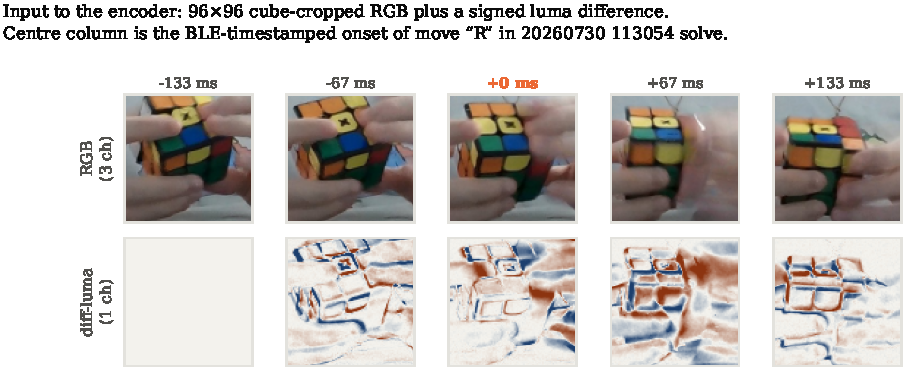
\includegraphics[width=\linewidth]{figures/fig_input.pdf}
\caption{The encoder's input on five consecutive held-out frames spanning
one ground-truth turn. Top: the cube-cropped colour channels. Bottom: the
signed luma difference (blue negative, orange positive). The first
difference panel is flat because the cube was genuinely still 133\,ms before
the turn --- that is the signal, not a rendering artefact. Note that the
turn is visible in the difference channel two frames \emph{before} the BLE
timestamp, which is the ${\sim}1$-frame label jitter discussed in
\cref{sec:labelnoise}.}
\label{fig:input}
\end{figure}

\paragraph{Crop-regime provenance.} The crop mode used to build each stream
is recorded inside the stream file and checked at train, eval and inference
time. This guard exists because of a real and expensive failure: for a
period the trainer silently fell back to \emph{uncropped} full frames for
sessions that lacked a cached crop, while inference always cropped. The
resulting evaluation compared a full-frame-trained model against
cropped-input test data and reported a 61.5\% aggregate that was really
90.6\% once the evaluation was made consistent. Nothing about the models had
changed. The lesson generalises past this project: \emph{when a retrain
appears to fix a regime, check what else changed about the data before
crediting the fix to the thing you meant to change.}

\subsection{The label frame problem}
\label{sec:labelframe}

The smart cube names turns relative to its own core. A middle-slice turn
(\wca{M}, \wca{E}, \wca{S}) --- which speedcubers perform constantly, and
which the cube reports as a pair of outer-layer turns --- rotates that core.
From that moment the cube's frame has rotated away from the camera's, and
every subsequent label names the wrong face. Two slices (\wca{M2}, common in
last-layer algorithms) and the cube calls the physically-top face \wca{D}
while the camera correctly sees \wca{U}.

This hid for a long time for an instructive reason. The repository's
session-consistency check applies each label to a \emph{cubie} model, which
has no centres and is therefore centre-relative by construction. It
validates the cube-frame product and is structurally blind to camera-frame
drift. It reported 16/16 sessions consistent throughout.

\begin{keybox}
\textbf{Never read a passing endpoint check as evidence about the frame of
reference.} A check that composes labels into a group element cannot see a
relabelling that composes to the identity, and the drift here \emph{does}
cancel: every affected session returns to identity by the end.
\end{keybox}

Scope: \SliceSessions\ sessions in the corpus contain slices, and because the drift
cancels, only \SliceMoves\ moves corpus-wide are actually misnamed
($\SliceMovePct$\%). It is a correctness fix, not an accuracy lever. But it
is still live in the repository: \emph{every} evaluation harness in
\file{ble/move\_detector/} scores against the cube-frame name, while
\file{prepare\_data.py} has trained against the camera-frame name since
2026-08-03. All measurements in this report use the camera frame.
\cref{sec:frame-result} quantifies the difference: on the three
slice-bearing held-out sessions it is worth $\FrameGainSlice$ points, and
$\FrameGainAll$ points averaged over the whole holdout.

\subsection{Label noise}
\label{sec:labelnoise}

Even without slices the labels are not exact. Aligning BLE timestamps to
frame timestamps gives a median offset of 6--10\,ms with a maximum around
33\,ms, i.e.\ up to one frame. This is irreducible at 30\,fps and is one
reason an order-only objective (CTC) is a better fit than an alignment
objective: CTC's loss is invariant to it, whereas Gaussian-target
supervision is asked to place a peak on the wrong frame roughly half the
time.

\subsection{Corpus and holdout policy}
\label{sec:holdout-hygiene}

The corpus is \NSessionsFrames\ sessions with usable frames across
\NDays\ distinct days, \NMovesTotal\ labelled turns, one solver, one cube,
two rooms. Sessions come in pairs: a \emph{scramble} take (a
machine-generated ${\sim}20$-move sequence performed slowly from a printed
prompt --- every move known exactly) and a \emph{solve} take (a free solve;
long, fast, and the regime that matters).

\paragraph{The holdout rule used here.} A session is evaluable for a
checkpoint if and only if its name appears in neither that checkpoint's
recorded \texttt{train\_session\_names} nor its
\texttt{val\_session\_names}. When several checkpoints are compared, the
holdout is the \emph{intersection} across all of them. This is computed from
the checkpoint files themselves, not from a maintained list.

Validation sessions are excluded on purpose. They chose the stopping epoch,
so they are model-selection data; in this corpus they are also same-day
neighbours of training sessions, which makes them the most flattering
sessions available. \cref{sec:ladder} measures exactly how flattering.

\paragraph{Where this differs from the repository's own numbers.} The
repository quotes results on ``the 8 never-trained \texttt{*\_solve}
sessions''. Two of those eight are the checkpoints' validation sessions.
Under this report's rule the equivalent set is \NHoldoutSolves\ solves ---
larger, because I prepared \NewlyPrepared\ sessions that had been recorded
but never run through preprocessing, and therefore had never been evaluated
by anything.

\begin{table}[t]
\centering\small
\caption{The evaluation set. Every session listed is absent from both the
training and validation lists of every checkpoint scored in this report.}
\label{tab:holdout}
\begin{tabular}{@{}llrrrrl@{}}
\toprule
session & clock & frames & turns & turns/s & crowded & regime \\
\midrule
07-29\,22:18 scramble & 22h & 803 & 20 & 0.79 & 0\% & evening \\
07-29\,22:18 solve & 22h & 1566 & 152 & 3.08 & 23\% & evening \\
07-30\,11:19 scramble & 11h & 880 & 20 & 0.79 & 0\% & daytime \\
07-30\,11:19 solve & 11h & 1464 & 106 & 2.23 & 10\% & daytime \\
07-30\,11:30 scramble & 11h & 964 & 20 & 0.65 & 0\% & daytime \\
07-30\,11:30 solve & 11h & 1545 & 132 & 2.72 & 16\% & daytime \\
07-31\,21:10 scramble & 21h & 863 & 20 & 0.76 & 0\% & evening \\
07-31\,21:10 solve & 21h & 1123 & 84 & 2.55 & 24\% & evening \\
07-31\,21:35 scramble & 21h & 1048 & 20 & 0.59 & 0\% & evening \\
07-31\,21:35 solve & 21h & 1215 & 108 & 2.88 & 19\% & evening \\
08-03\,09:51 scramble & 09h & 1012 & 22 & 0.67 & 0\% & daytime \\
08-03\,09:51 solve & 09h & 1062 & 82 & 2.58 & 17\% & daytime \\
08-03\,09:55 scramble & 09h & 993 & 20 & 0.68 & 0\% & daytime \\
08-03\,09:55 solve & 09h & 1849 & 140 & 2.38 & 14\% & daytime \\
08-03\,10:01 scramble & 10h & 767 & 20 & 0.90 & 0\% & daytime \\
08-03\,10:01 solve & 10h & 1458 & 123 & 2.93 & 24\% & daytime \\
08-03\,12:29 scramble & 12h & 1146 & 22 & 0.67 & 0\% & daytime \\
08-03\,12:29 solve & 12h & 1345 & 120 & 2.86 & 17\% & daytime \\
08-03\,12:34 scramble & 12h & 1028 & 22 & 0.66 & 0\% & daytime \\
08-03\,12:34 solve & 12h & 1015 & 88 & 2.81 & 17\% & daytime \\
08-04\,21:42 scramble & 21h & 940 & 20 & 0.67 & 0\% & evening \\
08-04\,21:42 solve & 21h & 1625 & 116 & 2.21 & 15\% & evening \\
08-04\,23:49 scramble & 23h & 857 & 20 & 0.74 & 0\% & evening \\
08-04\,23:49 solve & 23h & 1205 & 92 & 2.42 & 19\% & evening \\
08-05\,15:58 scramble & 15h & 943 & 20 & 0.66 & 0\% & daytime \\
08-05\,15:58 solve & 15h & 1512 & 124 & 2.70 & 17\% & daytime \\
08-09\,15:57 scramble & 15h & 803 & 20 & 0.81 & 0\% & daytime \\
08-09\,15:57 solve & 15h & 884 & 88 & 3.54 & 18\% & daytime \\
\bottomrule
\end{tabular}

\end{table}

\paragraph{The corpus is drifting, and that is measurable.} The solver got
roughly twice as fast over the three weeks of recording
(\cref{fig:drift}). The fraction of adjacent turn pairs within two frames
rose from under 1\% to \CrowdedPctHoldout\% in the held-out set. The
training corpus is therefore not merely small, it is weighted toward a
regime the solver has left. This confounds any attempt to read the
day-distance effect in \cref{sec:ladder} as pure generalisation: the more
distant sessions are also the faster ones.

\begin{figure}[t]
\centering
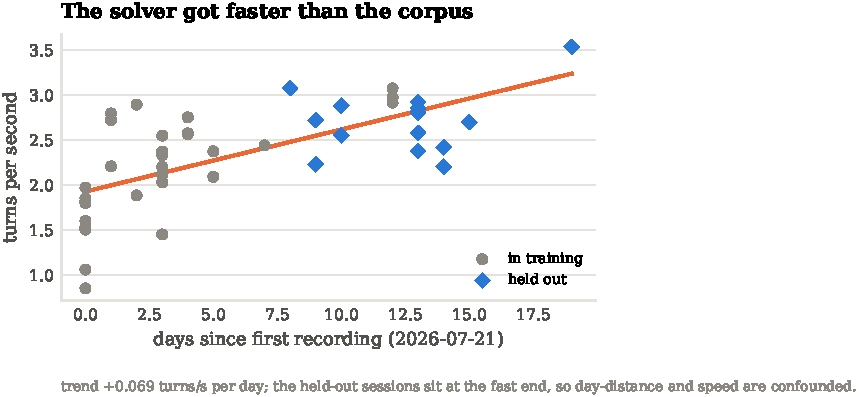
\includegraphics[width=0.86\linewidth]{figures/fig_drift.pdf}
\caption{Turn rate against recording date, every session with more than 40
turns. The held-out sessions are not a random sample of the corpus --- they
are systematically at the fast end, because they are the later ones. Any
claim of the form ``held-out accuracy is lower because the model does not
generalise across days'' is confounded with ``held-out accuracy is lower
because those solves are faster''.}
\label{fig:drift}
\end{figure}

\section{The recognition model}
\label{sec:model}

\begin{figure}[t]
\centering
% Architecture / dataflow diagram.
% Requires: tikz with arrows.meta, positioning (loaded in main.tex).
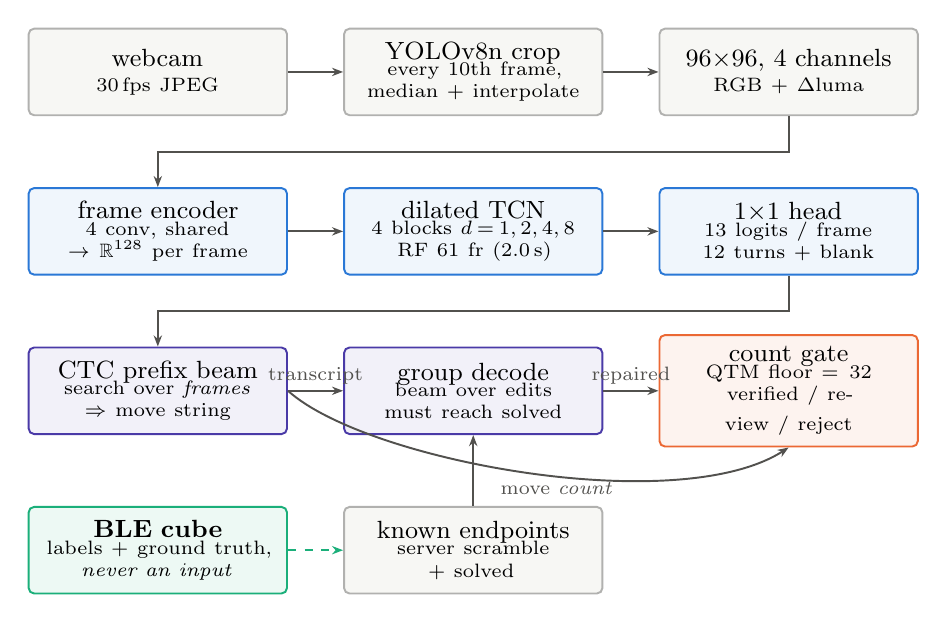
\begin{tikzpicture}[
  font=\small,
  box/.style={draw=prule, fill=white, rounded corners=2pt, line width=0.7pt,
              minimum height=11mm, text width=30mm, inner sep=4pt,
              align=center},
  learned/.style={box, draw=pblue, fill=pblue!7},
  search/.style={box, draw=pviolet, fill=pviolet!7},
  data/.style={box, draw=pgrey!45, fill=pbox},
  gate/.style={box, draw=porange, fill=porange!8},
  ar/.style={-{Stealth[length=4pt]}, draw=pgrey, line width=0.7pt},
  lbl/.style={font=\scriptsize, color=pgrey, inner sep=2pt},
]

% row 1 --- capture and preprocessing
\node[data]                          (cam)   at (0,0)      {webcam\\[-2pt]\scriptsize 30\,fps JPEG};
\node[data, right=7mm of cam]        (yolo)                {YOLOv8n crop\\[-2pt]\scriptsize every 10th frame,\\[-3pt]\scriptsize median $+$ interpolate};
\node[data, right=7mm of yolo]       (stack)               {$96{\times}96$, 4 channels\\[-2pt]\scriptsize RGB $+$ $\Delta$luma};

% row 2 --- the network
\node[learned, below=9mm of cam]     (enc)                 {frame encoder\\[-2pt]\scriptsize 4 conv, shared\\[-3pt]\scriptsize $\to\mathbb{R}^{128}$ per frame};
\node[learned, right=7mm of enc]     (tcn)                 {dilated TCN\\[-2pt]\scriptsize 4 blocks $d\!=\!1,2,4,8$\\[-3pt]\scriptsize RF 61 fr ($2.0$\,s)};
\node[learned, right=7mm of tcn]     (head)                {$1{\times}1$ head\\[-2pt]\scriptsize 13 logits / frame\\[-3pt]\scriptsize 12 turns $+$ blank};

% row 3 --- the two searches and the gate
\node[search, below=9mm of enc]      (beam)                {CTC prefix beam\\[-2pt]\scriptsize search over \emph{frames}\\[-3pt]\scriptsize $\Rightarrow$ move string};
\node[search, right=7mm of beam]     (recon)               {group decode\\[-2pt]\scriptsize beam over edits\\[-3pt]\scriptsize must reach solved};
\node[gate,   right=7mm of recon]    (gate)                {count gate\\[-2pt]\scriptsize QTM floor $=32$\\[-3pt]\scriptsize verified / review / reject};

% row 4 --- side inputs
\node[data, below=9mm of beam, draw=paqua, fill=paqua!8] (ble)
      {\textbf{BLE cube}\\[-2pt]\scriptsize labels + ground truth,\\[-3pt]\scriptsize \emph{never an input}};
\node[data, below=9mm of recon]      (states)              {known endpoints\\[-2pt]\scriptsize server scramble\\[-3pt]\scriptsize $+$ solved};

% arrows
\draw[ar] (cam)   -- (yolo);
\draw[ar] (yolo)  -- (stack);
\draw[ar] (stack.south) -- ++(0,-4.5mm) -| (enc.north);
\draw[ar] (enc)   -- (tcn);
\draw[ar] (tcn)   -- (head);
\draw[ar] (head.south)  -- ++(0,-4.5mm) -| (beam.north);
\draw[ar] (beam)  -- node[lbl, above]{transcript}   (recon);
\draw[ar] (recon) -- node[lbl, above]{repaired}     (gate);
\draw[ar] (states.north) -- (recon.south);
\draw[ar, draw=paqua, dashed] (ble.east) -- (states.west);
\draw[ar] (beam.east) .. controls +(10mm,-9mm) and +(-14mm,-9mm)
          .. node[lbl, below, pos=0.55]{move \emph{count}} (gate.south);

\end{tikzpicture}

\caption{The pipeline. Everything left of the dashed line is per-frame and
learned; everything right of it is a search. The smart cube (bottom) supplies
labels during data collection and ground truth during evaluation, and is
absent at inference.}
\label{fig:pipeline}
\end{figure}

\subsection{Architecture}
\label{sec:arch}

The network is deliberately small: \NParams\ parameters, trained in minutes,
chosen so that ``wrong architecture'' and ``not enough data'' stay
distinguishable. With ${\sim}5{,}000$ labelled turns from one person, a large
recurrent model over raw frames has ample capacity to memorise grip and
lighting.

\paragraph{Frame encoder.} Four strided $3\times3$/$5\times5$ convolutions
with batch-norm and ReLU take $4\times96\times96 \rightarrow 128\times6\times6$,
followed by global average pooling: one 128-dimensional vector per frame,
weights shared across frames. Pooling away the spatial dimensions is a real
commitment --- it discards \emph{where} on the cube the motion was --- and it
is defensible only because the temporal difference channel already encodes
the pattern of a turn rather than its location. It is also the most obvious
thing to revisit (\cref{sec:gap}).

\paragraph{Temporal convolutional network.} Four residual blocks, each two
$3$-wide dilated 1-D convolutions at dilations $1,2,4,8$ with `same' (centred)
padding. The receptive field is
\begin{equation}
1 + \sum_{d\in\{1,2,4,8\}} 4d \;=\; 61 \text{ frames} \;\approx\; 2.03\,\text{s
at 30\,fps,}
\end{equation}
i.e.\ each output frame sees roughly one second either side. The network is
therefore \textbf{non-causal by design}, which suits the intended product
flow (buffer the solve, analyse it afterwards) and would need causal padding
and an accuracy sacrifice at the leading edge for true streaming.

\paragraph{Heads.} A $1\times1$ convolution maps the 128-channel trunk to 13
logits per frame: 12 quarter turns plus blank. A second $1\times1$ head
producing a single onset logit is retained from the earlier architecture and
is trained with weight $0$ in the shipped configuration; it is what the
peak-picking arm in \cref{sec:ablation} uses.

Being fully convolutional in time means the model trains on fixed-length
clips and runs a whole session in one pass. In practice a session is chunked
at 480 frames with 30 frames of context on each side that are then
discarded, because a chunk boundary with zero padding produces a band of
${\sim}60$ unreliable scores --- over 10\% of a session's output, exactly
where symbols are being read off.

\subsection{Two supervision regimes}
\label{sec:supervision}

The same trunk was trained two ways, and the difference is the most
consequential design decision in the project.

\paragraph{(a) Alignment supervision.} Each BLE onset becomes a Gaussian
bump ($\sigma = 1$ frame) in a per-frame target; the onset head is trained
with BCE, the class head with cross-entropy at labelled frames. At inference,
peaks are picked out of the onset score (threshold, minimum separation), each
peak becomes a move, and the class head is read at the peak frame.

\paragraph{(b) CTC.} The 13th column becomes a blank, the loss is
$-\log p(\ell^\star \mid x)$ from \cref{eq:ctcmarginal}, and nothing ever
tells the network \emph{where} a move was.

Regime (a) uses information that regime (b) throws away, which sounds like a
straightforward advantage. The argument for (b) is that the discarded
information is \emph{partly wrong exactly where the pipeline fails}:
\CorpusCrowdedTwo\% of turns land within two frames of a neighbour and
\CorpusSameFrame\% cannot be assigned distinct frames at all
(\cref{sec:capture}), and those crowded pairs are the same population that
peak-picking loses to merged humps. CTC is indifferent to both.

\paragraph{The deeper problem with (a) is architectural, not statistical.}
Peak-picking commits to a discrete candidate list \emph{before} any
downstream search runs. Every phantom and every miss in the pipeline is
created at that one line. A regrip hump that clears the threshold becomes a
phantom the group decoder must pay to delete; two onsets closer than the
minimum separation can never both be reported at all. CTC does not improve
that step, it removes it: the search runs over \emph{frames}, so ``is there a
move here'' is decided inside the search, weighed against everything else,
rather than greedily beforehand by a constant.
\Cref{sec:ablation} measures the swap.

\subsection{What the model actually emits}
\label{sec:posteriorgram}

\begin{figure}[t]
\centering
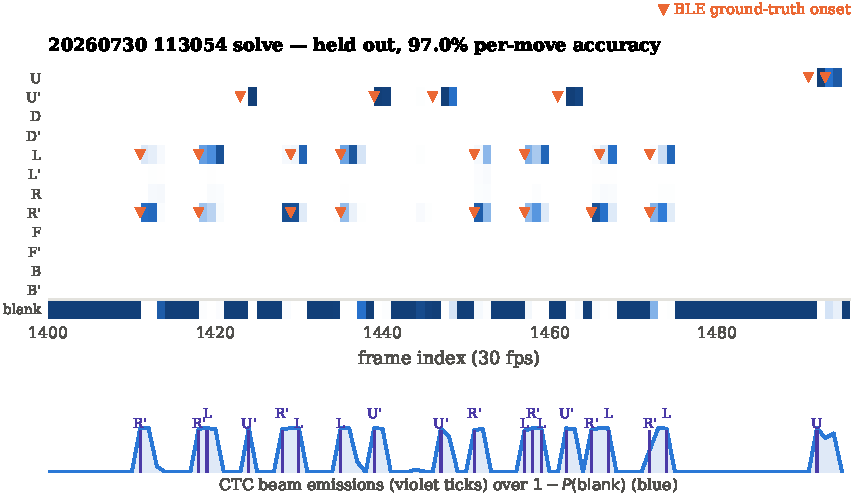
\includegraphics[width=\linewidth]{figures/fig_posteriorgram.pdf}\\[6pt]
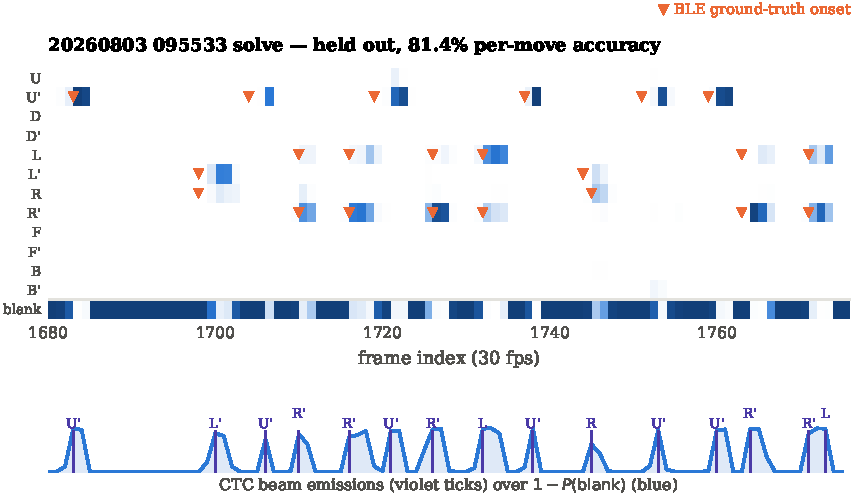
\includegraphics[width=\linewidth]{figures/fig_ctc_failure.pdf}
\caption{The 13-way per-frame posterior over 3.2\,s of two held-out
sessions, with BLE ground-truth onsets marked. \textbf{Top:} a session the
model reads well. The posterior is extremely peaky --- the network spends
${\sim}90$\% of frames confidently in blank and commits for one or two frames
per turn --- and every truth marker has a matching dark cell in its own row.
\textbf{Bottom:} a session it reads badly. The posterior is visibly softer
and several truth markers sit over rows with no committed mass at all;
those are the misses that dominate the error budget. Note in both panels
that emissions do not have to align with the markers, only to appear in the
right order: CTC is never told where a move was.}
\label{fig:posteriorgram}
\end{figure}

\Cref{fig:posteriorgram} is the most useful single picture of this system.
Two properties are worth reading off it.

First, \textbf{CTC produces a peaky posterior}, not a smooth one. This is a
well-known property of the objective --- the marginalisation in
\cref{eq:ctcmarginal} is happy to place all of a symbol's probability on one
frame --- and it has a practical consequence: the ``score'' of a move is not
a smooth confidence that can be thresholded, which is why the decoders in
\cref{sec:decode} search over frames rather than over thresholded peaks.

Second, \textbf{the failure mode is silence, not confusion}. In the lower
panel the model does not name turns wrongly so much as decline to name them.
That is consistent with the error decomposition in \cref{sec:main-results}
and it is why the group decoder --- whose cheap repair is substitution ---
has so little to work with.

\subsection{Augmentation}
\label{sec:aug}

Two families, both applied per clip.

\paragraph{Photometric.} Gain $\in[0.55,1.60]$, offset $\pm 30$, gamma
$\in[0.60,1.65]$, per-channel white balance $\in[0.86,1.16]$, saturation
$\in[0.65,1.35]$, per-frame gain wobble ($\sigma=0.03$), Gaussian noise
($\sigma$ up to 5), and with probability $0.15$ a 3-frame temporal box blur
simulating the longer exposure of a dim room. These ranges are roughly
3--4$\times$ wider than the original ones, widened after an evening take
scored 56\% against ${\sim}91\%$ on two morning takes.

\paragraph{Speed.} With probability $0.5$ a clip is time-warped by a factor
in $[1.2, 3.0]$, resampling $96\cdot s$ source frames down to 96. On a
2.4\,turns/s corpus a factor of 3 reaches ${\sim}7$\,turns/s.

Speed augmentation was introduced for an anticheat reason --- the count gate
needs the model not to under-count fast solves --- and the repository records
it as having ``zero validation cost''. \Cref{sec:ablation} shows that on a
never-seen holdout it is the largest single accuracy intervention on record.
This is the sharpest instance in the project of a recurring lesson:
\emph{validation MER did not rank these interventions, and the corpus's own
validation split was structurally incapable of doing so} because it is
same-day adjacent (\cref{sec:ladder}).

One practical note that cost a debugging session: with speed augmentation the
CTC loss escapes its all-blank plateau roughly four epochs later than
without. That is expected --- time-warped clips make the alignment problem
harder early --- and is not a bug, but it looks exactly like one.

\subsection{Training}

AdamW, learning rate $3\times10^{-4}$, weight decay $10^{-2}$, batch 8 clips
of 96 frames (3.2\,s) sampled at stride 24, gradient clipping at 5, mixed
precision, 60 epochs with patience 15. Model selection is by move error rate
on the held-out validation sessions, never by loss: per-frame loss is
dominated by the easy blank frames between moves, and a model can improve
its loss while getting worse at emitting exactly one symbol per turn.

\textbf{Session-level holdout is mandatory}, not optional. Clips from one
session overlap and share lighting, grip and background; a random clip split
reports memorisation. Every checkpoint in this report was trained with named
validation sessions.

Two seeds are trained for every configuration and both are always reported.
The two-seed spread on this metric is 0.5--3 points depending on regime, and
several interventions in the project's history were smaller than it.

\section{Decoding}
\label{sec:decode}

There are two searches, and conflating them is the single most common source
of confusion about this system. The first turns a posteriorgram into a move
string. The second turns a move string into a move string that is
\emph{algebraically possible}. They have different objectives, different
failure modes, and --- crucially --- different standing as evidence.

\subsection{Why not peak-picking}
\label{sec:peakpick}

The obvious decoder for a per-frame onset score is: threshold, find local
maxima at least $m$ frames apart, emit one move per maximum, read the class
head at that frame. It has three failure modes, all of which were measured.

\begin{enumerate}[leftmargin=1.4em,itemsep=2pt]
\item \textbf{Merged humps.} Two turns closer than $m$ frames become one
symbol. Raising $m$ loses fast pairs; lowering it invents phantoms in the
shoulders of a single hump. In this corpus 34\% of sub-150\,ms pairs arrive
as one merged hump at the tuned operating point.
\item \textbf{Constants tuned on the wrong regime.} $m$ and the target width
$\sigma$ were both tuned on 2026-07-21 footage containing almost no fast
moves (2.5\% of pairs under 100\,ms). Against footage where 28\% of onsets
have a neighbour under 150\,ms, retuning $m: 3\to2$ and $\sigma: 2\to1$ moved
sub-150\,ms recall from 73.8\% to 83.5\%. \emph{A decoder constant tuned on
one speed regime silently becomes a ceiling in another, and from the outside
it looks exactly like a model limitation.}
\item \textbf{Premature commitment.} The candidate list is fixed before any
downstream evidence is consulted. This is the structural objection and it is
not fixable by tuning.
\end{enumerate}

\subsection{CTC prefix beam search}
\label{sec:prefixbeam}

The decoder must approximate
$\hat\ell = \arg\max_\ell p(\ell\mid x)$ where $p(\ell \mid x)$ is the sum
over alignments in \cref{eq:ctcmarginal}. Best-path decoding (per-frame
argmax, then collapse) maximises the probability of a single \emph{path},
which is a different thing, and the two differ exactly when the model is
uncertain --- which is the regime of interest. \cref{sec:main-results}
measures the gap: \GreedyGap\ points.

Prefix beam search \cite{hannun2014} maintains a set of prefixes, each
carrying two accumulators:
\begin{align}
p_b(\ell, t) &= \Pr[\text{paths over frames } 1{:}t
   \text{ that collapse to } \ell \text{ and end in blank}],\\
p_{nb}(\ell, t) &= \Pr[\text{same, ending in a non-blank symbol}].
\end{align}
The split exists to express the repeat rule. Extending prefix $\ell$ by
symbol $c$ at frame $t$:
\begin{equation}
p_{nb}(\ell c, t) \mathrel{+}= y^t_c \cdot
\begin{cases}
p_b(\ell, t-1) & \text{if } c = \mathrm{last}(\ell),\\
p_b(\ell,t-1) + p_{nb}(\ell,t-1) & \text{otherwise,}
\end{cases}
\label{eq:extend}
\end{equation}
because a repeat of the last symbol only creates a \emph{new} emission if
the previous frame was blank; otherwise it merely extends the existing
emission, which contributes to $p_{nb}(\ell,t)$ rather than to
$p_{nb}(\ell c,t)$. Staying blank carries $\ell$ forward:
$p_b(\ell,t) \mathrel{+}= y^t_\varnothing (p_b(\ell,t-1)+p_{nb}(\ell,t-1))$.
Prefixes are ranked by $\log(p_b+p_{nb})$ and pruned to the beam width (16
here). Everything is in log space: over a 1600-frame session, linear
probabilities underflow within a few hundred frames and the beam silently
degenerates to whatever ties at zero.

\paragraph{Frames are approximate.} A prefix is reached by many alignments
that disagree about which frame emitted which symbol, so each prefix keeps
the frame list of its single largest contribution. Nothing downstream uses
those frames for cost --- only for ordering and reporting --- so the
approximation never enters a score.

\paragraph{Language-model fusion, and why it is off.} Shallow fusion,
$\mathrm{rank}(\ell) = \log p_{\text{ctc}}(\ell) + \alpha \log
p_{\text{lm}}(\ell) + \beta|\ell|$, was implemented and measured. It helps
consistently across days (MER $17.3\to9.8$ and $17.1\to12.2$ by seed) and
\emph{flips sign} on the same-day validation split, because one global
$\beta$ cannot serve both regimes. It is off by default. The $\beta$ term is
not a hack: any language model systematically prefers shorter sequences, so
without an explicit per-symbol insertion bonus, fusion trades phantoms for
misses rather than reducing error.

\subsection{What CTC's independence assumption costs}
\label{sec:ctc-limits}

\Cref{eq:pathprob} factorises the path probability across frames, which
means the model has \emph{no} way to express ``having just emitted
\wca{R}, \wca{R'} is now unlikely''. All sequence-level structure has to be
carried implicitly by the trunk's receptive field --- 61 frames, about two
seconds, or roughly five turns at the corpus's median rate. Anything longer
range than that is invisible to the objective.

For this domain that is a real limitation, because the output has enormous
long-range structure: the last third of a solve is drawn from a repertoire
of a few dozen memorised words, and a solver's move distribution is far from
i.i.d. Two remedies exist and both were tried.

\begin{itemize}[leftmargin=1.3em,itemsep=2pt]
\item \emph{Shallow fusion with a move language model} (above). Helps
cross-day, hurts same-day, sign-unstable --- off by default.
\item \emph{An explicit algorithm prior} in the group decoder --- recognise a
known last-layer word and insert it as a single beam transition. Measured
inert in the forward direction and net negative in the backward direction
(\cref{sec:negatives}).
\end{itemize}

The honest reading is that neither failed because sequence structure is
absent --- it is obviously present --- but because both were applied
\emph{after} the frame-level model had already lost the evidence. A model
that conditions on its own emission history (an RNN-transducer or an
attention decoder) would carry the prior where it can still change what is
recognised. That is the most defensible architectural change available and
it has not been tried.

\subsection{The group-theoretic decode}
\label{sec:reconstruct}

\paragraph{Setup.} We have a start state $s_0 \in G$ (the server-issued
scramble, known exactly), an end state (solved, $e$), and a detected
sequence of $n$ onsets, each with a 12-way posterior $p_j$ over classes.
We want the most probable move word $w$ such that $s_0 \cdot w = e$.

Model the recogniser as a noisy channel with three error types --- the
alignment operations of \cref{sec:experiments}: a \emph{substitution} (onset
detected, named wrong), a \emph{phantom} (spurious onset), a \emph{miss}
(onset never emitted). A hypothesis is a sequence of edit decisions; its cost
is a sum of negative log-probabilities, so minimising cost is MAP estimation.

\paragraph{The cost model.} For onset $j$, accepting class $k$ costs
\begin{equation}
c_j(k) \;=\; \log \max_i q_j(i) \;-\; \log q_j(k),
\qquad
q_j \;=\; (1-\rho_j)\,p_j \;+\; \tfrac{\lambda_u}{12}\mathbf{1}
        \;+\; \lambda_i u_j\, \delta_{\mathrm{inv}(\arg\max p_j)},
\label{eq:acceptcost}
\end{equation}
where $u_j = 1 - \max_i p_j(i)$ is the onset's uncertainty and
$\rho_j = \lambda_i u_j + \lambda_u$. Accepting the model's own argmax is
free by construction; everything else is priced by how far the smoothed
posterior falls short of it. Two smoothing terms are added because the raw
softmax is badly calibrated in a specific, measured way: it is overconfident
precisely on the temporal inverse (\wca{U} versus \wca{U'}), so
$\lambda_i = 0.20$ of prior mass, scaled by the onset's own uncertainty, is
moved onto the inverse class, plus a flat $\lambda_u = 0.04$ uniform floor.

Deleting onset $j$ (declaring it a phantom) costs
$C_{\mathrm{del}} + w\cdot(\text{onset strength})$ with
$C_{\mathrm{del}}=2.6$. Making deletion depend on strength is not a
refinement, it is load-bearing: with a flat deletion cost the beam drowns in
``delete something here, insert something there'' pairs --- there are
$O(n^2\cdot 12)$ of them, they are parity-balanced, and they are all cheaper
than a true multi-substitution story. Onset strength is genuine evidence
against deletion and pricing it removes the flood.

Inserting a move (recovering a miss) costs a flat $C_{\mathrm{ins}} = 4.0$,
roughly $-\log$ of the miss odds plus the 12-way choice of which move.

\paragraph{Why beam search and not exact search.} At the measured error rate
an exact IDA* over edit cost is hopeless, because the constraint that kills
wrong hypotheses --- ``does this reach solved'' --- only pays off at the
\emph{end} of the sequence. At a budget sufficient for ten edits the tree
explodes long before pruning bites. So: keep the $K$ cheapest hypotheses per
onset ($K = 4000$, retried at $16000$), deduplicated by cube state, ranked
by cost-so-far plus an admissible lookahead.

\paragraph{The lookahead.}
\label{sec:heuristic}
Three components, two of them true lower bounds.
\begin{itemize}[leftmargin=1.3em,itemsep=2pt]
\item \emph{Pattern databases.} Breadth-first tables over the corner-twist,
edge-flip and UD-slice coordinates give an admissible quarter-turn distance
from any state to solved; the max over tables is used.
\item \emph{Parity.} Every quarter turn flips permutation parity
(\cref{sec:background}), so a hypothesis whose achievable remaining move
count has the wrong parity provably needs a further insertion or deletion.
\item \emph{A suffix-consistency ladder.} This one is the interesting part.
Precompute $S_j$, the group product of the \emph{remaining} detected moves as
classified. A hypothesis is consistent with the rest of the detections iff
$\mathrm{rel} = \mathrm{state}\cdot S_j$ is the identity. Grading ``almost
consistent'' by pattern distance does \emph{not} work --- a conjugated error
scrambles the coordinate metrics, so $h(\mathrm{rel})$ measures $20\pm3$ for
\emph{any} hypothesis with at least one unfixed error regardless of how many,
and feeding that noise into the ranking evicts the true hypothesis. What
works is exact algebra: $\mathrm{rel}$ is repairable by one future insertion
of $m$ at gap $q$ iff $\mathrm{rel} = S_q^{-1} m^{-1} S_q$, by one future
deletion of detection $q$ iff $\mathrm{rel} = S_{q+1}^{-1} d_q S_{q+1}$, and
by one future substitution of $m$ for $d_q$ iff
$\mathrm{rel} = S_{q+1}^{-1}(m^{-1}d_q)S_{q+1}$. Those $\sim\!25n$ elements
go into a hash set; the ranking adds a weight per ``level'' (0 = consistent
now, 1 = one edit away, capped otherwise). It is noise-free, and the moment a
hypothesis has repaired everything but one discrepancy it out-ranks the
cheap procrastinators an absolute-cost beam would bury it under. It is a
ranking term, never a hard prune.
\end{itemize}

\paragraph{The tail is exact.} After the last onset, each candidate end state
is finished by iterative-deepening search over words of length
$\le M_{\mathrm{end}} = 4$, pruned by the full pattern-database bound. This
covers end-of-solve moves the camera never saw. \textbf{The small budget is
what keeps the whole thing sound}: every state is within 26 quarter turns of
solved, so with a generous budget \emph{every} branch ``verifies'' and the
result means nothing.

\subsection{What the group decode can and cannot repair}
\label{sec:decode-limits}

The endpoint constraint is \emph{global and terminal}. It discriminates
nothing until the last onset. A session that cannot complete a consistent
path to solved therefore receives only generic smoothing, and all of the
decode's power concentrates in sessions that were nearly right already. This
is why the measured contribution is about a point (\cref{sec:decode-results})
rather than the large number the framing suggests.

Per channel:
\begin{itemize}[leftmargin=1.3em,itemsep=2pt]
\item \textbf{Substitutions} are the channel the constraint fixes nearly for
free --- the group pins down which move a mis-named onset must have been. It
is also the \emph{smallest} channel (\SubShare\% of error mass).
\item \textbf{Phantoms} are cheap to delete when the onset was weak.
\item \textbf{Misses} force the decoder to invent a move with no posterior
evidence at all: a 12-way guess whose only support is an endpoint dozens of
moves away. They are \MissShare\% of the error mass, i.e.\ most of it.
\end{itemize}

The envelope is best stated in \emph{cost}, not error count, because cost is
what actually binds. Measured on synthetic corruptions and on a real replay:
a true story costing ${\sim}6$ survives 90 onsets at beam 4000; one costing
${\sim}10$ does not, and each insertion is a flat 4.0. So there is roughly
\emph{one insertion of headroom beyond whatever the recogniser's own mistakes
already cost.} Buying down recognition error buys miss recovery for free;
widening the beam does not.

That envelope is the whole story of \cref{sec:decode-results}: on the
held-out set the cheapest true story costs \MinGtPathCost\ and the median
costs \MedGtPathCost, so nothing is within reach and the decode's measured
contribution is \DecodeGain\ points. A decoder with exactly one anchor, at
the very end, cannot help a sequence that needs a dozen insertions to reach
it.

\section{Verification, and what a verdict is worth}
\label{sec:verification}

\subsection{The separation of concerns that took longest to get right}

For most of this project's life, ``verify a solve'' meant ``reconstruct the
move sequence exactly enough that it provably reaches solved''. That framing
is wrong, and the reason is worth stating carefully because it is the
conceptual core of the whole system.

Reconstruction accuracy and legitimacy are different questions, and the
first is a \emph{terrible} instrument for the second.

\begin{keybox}
\textbf{Verification is a cliff.} Empirically, sessions above ${\sim}98\%$
raw per-move accuracy reconstruct exactly and verify; sessions in the 95--98\%
band verify essentially never (0 of 4 in the recorded corpus). There is no
graded middle. So a legitimacy test built on exact reconstruction rejects
honest users for being filmed in slightly worse light --- it is a
\emph{model-quality} test wearing a legitimacy test's clothes.
\end{keybox}

The system therefore splits into two tiers with different jobs:

\begin{description}[leftmargin=1.2em,style=nextline,itemsep=3pt]
\item[The accuracy tier (the group decode).] Makes the recorded transcript as
close to what was performed as possible. Its output is a product feature
(coaching, move-by-move review). It issues no verdicts.
\item[The legitimacy tier (the count gate).] Decides
\texttt{VERIFIED}/\texttt{REVIEW}/\texttt{REJECTED}. It uses only the
\emph{number} of moves, never their identity.
\end{description}

\subsection{Falsifiability: the measurement that makes a verdict mean
anything}
\label{sec:falsifiability-method}

A verifier that has only ever been run on genuine solves has not been
evaluated. \texttt{VERIFIED} is not a result until you know what the same
video says to a claim that is false.

So every decode is re-run against deliberately wrong claims, under an
\emph{identical} cost model: the same onsets, the same posteriors, the same
beam, decoded against a start state that is 1, 2 or 4 quarter turns away
from the truth, and against a cube that was never scrambled at all. A
verifier that accepts these is worthless; one that rejects them has
demonstrated something.

\paragraph{And here is the part that must not be oversold.} Suppose the true
claim decodes to word $W$ at cost $c(W)$. A claim whose start state is $d$
quarter turns away from the truth is solved by the word $w^{-1}W$, where $w$
is the offending $d$-move prefix. That word accepts exactly the same onsets
as $W$ and additionally performs $d$ insertions. So a valid story for the
false claim \textbf{provably exists} at cost
\begin{equation}
c(W) + d\cdot C_{\mathrm{ins}},
\label{eq:decoybound}
\end{equation}
whether or not the beam finds it. When the system rejects a 1-move-off
decoy, it is being rejected by the \emph{search}, not by the cost model,
whose own separation is only $C_{\mathrm{ins}} = 4.0$ per quarter turn of
claim error.

This is not hypothetical. On one session the 1-move-off decoy is rejected at
beam 4000 and at 16000, and \emph{accepted at beam 64000 at cost 10.17} ---
exactly $6.17 + C_{\mathrm{ins}}$, the constructive bound. Operationally the
system does reject near decoys at the deployed beam, which is what a
verifier has to do; but reporting that as evidence that no cheap wrong story
exists would be the easiest way to oversell this pipeline, and
\cref{eq:decoybound} says one does.

\subsection{The count gate}
\label{sec:count-gate}

\subsubsection{Threat model}

Everything physical reduces to three attacks, and naming them this way
matters because two of them are not swaps, so swap detection cannot see
them.

\begin{center}\small
\begin{tabular}{@{}clp{7.6cm}@{}}
\toprule
& \textbf{Attack} & \textbf{What can catch it} \\
\midrule
A & Substitution --- swap in a solved cube
  & move-count floor; frame-continuity guard; persistent appearance change \\
B & Solving outside the timed window --- follow a solver's output, or stop
    the timer unsolved and solve before scanning
  & move-count floor; the post-stop phantom-rate test \\
C & Video injection / virtual camera
  & \emph{nothing in the video}; challenge--response only \\
\bottomrule
\end{tabular}
\end{center}

\subsubsection{Why counting, and why the metric is the trap}

Move-by-move verification is dead (the cliff above). But that cliff is about
\emph{which} move. Counting discards substitutions entirely and is sensitive
only to insertions and deletions, so it runs on the model's strong axis. MER
is an over-estimate of counting error.

Attack A is defeated trivially: a swapped-in solved cube requires zero moves.
Attack B's first form is the interesting one --- run the scramble through a
solver and execute the answer. Every move genuinely happens; one cube is on
camera throughout; nothing is fake except the thinking.

But a solver's output is \emph{bounded} and a human method is not. So the
floor sits above the longest solution any solver would produce.

\begin{keybox}
\textbf{God's number is 20 in the half-turn metric. This alphabet has no
half-turn symbol}, so \wca{R2} decodes as \wca{R},\wca{R} and everything
here is quarter-turn metric, where God's number is \textbf{26}. A floor set
at ``twenty-something'' would sit \emph{below} the cheat ceiling and catch
nothing.
\end{keybox}

The operative ceiling is not 26 but 30: a cheat runs a two-phase solver, not
an optimal one, and two-phase returns ${\sim}19$--$22$ HTM $\approx 25$--$30$
QTM. The recorded scramble takes corroborate this at 20--28 QTM true.
Constants: solver ceiling 30 QTM, floor on observed moves 32, assumed
efficient-human floor 45 QTM.

\subsubsection{Calibration, and the abstain band}

The gate sees \emph{predicted} moves, and the model under-counts, more so the
faster the solve. Under-counting pushes a cheat further below the floor
(harmless) and a legit solve toward it (the false-DQ risk), so the floor must
be calibrated against worst-case retention, not mean. Retention is measured
by time-warping real sessions to a target turn rate and comparing decoded
count to true count. Taking the \emph{worse} of the two seeds at each level:
at 5\,turns/s retention is 0.88, at 8\,turns/s 0.80, at 10\,turns/s 0.69.

Above some rate the two bands genuinely overlap and no threshold separates
them. That limit is \emph{derived} from the floor rather than hardcoded, so
changing the floor moves it automatically; speed augmentation moved it from
7.11 to 9.62\,turns/s. At 9.62\,turns/s a 45-move solve takes 4.7\,s, against
a ${\sim}3.1$\,s world record --- so the ``too fast to read'' abstain case now
covers only the very fastest humans alive.

\subsubsection{Three tiers, and the order of the checks}

The gate returns \texttt{VERIFIED}, \texttt{REJECTED} or \texttt{REVIEW},
unlike the frame-continuity guard which is deliberately two-tier. Two
conditions here make the evidence \emph{unreadable} rather than
incriminating: too fast to separate, and bad light. Bad light matters
specifically because in low light the \emph{onset detector} loses 40+ points
while the classifier loses ${\sim}5$ --- and the count \emph{is} the
detector's output, so bad light would fabricate a ``too few moves'' rejection
out of a model failure. Abstain conditions are therefore checked
\textbf{before} reject conditions, so a solve is never rejected on evidence
that has just been declared unreadable.

\subsubsection{The hole that remains}

Stated plainly, because it is easy to believe the gate closed more than it
did. \textbf{Make a full solve's worth of plausible moves on camera without
solving, then swap in a solved cube.} That reads as ${\sim}50$ moves, clears
the floor of 32, and the count gate passes it --- eight seconds of flailing
suffices, which would be a world-class time. Nothing about the move count
distinguishes it from a real solve, because the move count is genuinely real;
only the outcome is faked. Frame continuity and appearance own this case
entirely, which is why the count gate can never be the only arm.

Camera injection (attack C) is not addressed by any video analysis. The
defence is protocol: server-issued unique scrambles mean a pre-recorded video
cannot match a fresh challenge, plus challenge--response (demand a specific
face at a random moment). Not built.

\section{Experiments}
\label{sec:experiments}

\subsection{Protocol}

Everything in this section was produced by \file{paper/scripts/} in one
sitting, on the machine described in \cref{app:repro}, from the checkpoints
\file{move\_ctc\_spd\_s0.pt} and \file{move\_ctc\_spd\_s1.pt} unless stated
otherwise. Rules, each of which has cost this project a wrong conclusion at
some point:

\begin{enumerate}[leftmargin=1.4em,itemsep=2pt]
\item \textbf{Both seeds, always.} The two-seed spread on this metric is
0.5--3 points and several historical ``improvements'' were smaller.
\item \textbf{Never pool a mean over moves when the claim is about
sessions.} The headline is a mean of per-session accuracies; a long solve
must not dominate a short one. Pooled numbers are reported separately where
they differ.
\item \textbf{Split by lighting regime, never pooled.} The pooled
distribution is bimodal and the pooled mean describes nothing.
\item \textbf{Re-run the baseline in the same sitting.} No number here is
compared against a value recalled from a document.
\item \textbf{Held-out means held out of training \emph{and} validation}
(\cref{sec:holdout-hygiene}).
\item \textbf{Resample sessions, not moves.} Confidence intervals are
bootstrapped over sessions ($20{,}000$ resamples), because the quantity
being estimated is ``what would this model score on a new session'', and
moves within a session are strongly dependent --- the $16\times$
per-session spread in miss rate \emph{is} that dependence. Resampling moves
would give intervals several times too narrow.
\item \textbf{Compare rungs pairwise.} Every ablation rung is scored on the
same \NPaired\ sessions, so the statistic is the mean per-session
\emph{difference}, tested with an exact sign test (no distributional
assumption at this $n$).
\end{enumerate}

The metric is per-move accuracy under Needleman--Wunsch alignment against the
camera-frame BLE word: alignment, not index-by-index comparison, because one
dropped move shifts every later index and a positional comparison would read
a single miss as ${\sim}25$ errors. The alignment's three non-match
operations are exactly the three failure modes: \emph{miss} (recall),
\emph{phantom} (precision), \emph{substitution} (naming). Move error rate
(Levenshtein distance over $|{\rm truth}|$) is reported alongside because it
charges phantoms, which accuracy does not.

\subsection{Main result: raw recognition}
\label{sec:main-results}

\begin{table}[t]
\centering\small
\caption{Raw CTC recognition on the never-seen holdout, mean of per-session
accuracies. The CTC ceiling column is the structural limit from
\cref{sec:ctc-bg} --- same-class onset pairs within two frames, which no
amount of training removes.}
\label{tab:main}
\begin{tabular}{@{}llrrrrr@{}}
\toprule
take type & regime & $n$ & moves & seed 0 & seed 1 & CTC ceiling \\
\midrule
solve & daytime & 9 & 1003 & 91.2\% & 90.2\% & 98.1\% \\
solve & evening & 5 & 552 & 85.2\% & 90.0\% & 99.1\% \\
solve & all & 14 & 1555 & 89.0\% & 90.2\% & 98.5\% \\
\midrule
scramble & daytime & 9 & 186 & 97.2\% & 97.2\% & 100.0\% \\
scramble & evening & 5 & 100 & 97.0\% & 96.0\% & 100.0\% \\
scramble & all & 14 & 286 & 97.1\% & 96.8\% & 100.0\% \\
\bottomrule
\end{tabular}

\end{table}

On \NHoldoutSolves\ free solves (\NHoldoutMoves\ turns) no checkpoint has
seen, per-move accuracy is \RawDaySA\%/\RawDaySB\% daytime and
\RawEveSA\%/\RawEveSB\% evening by seed, against a structural CTC ceiling
of \CTCCeilingHoldout\%. Averaging the seeds and bootstrapping over
sessions, that is \CIDayMean\% [\CIDayLo, \CIDayHi] daytime and
\CIEveMean\% [\CIEveLo, \CIEveHi] evening --- intervals wide enough that
the two regimes overlap, which is worth keeping in mind every time this
report calls the evening gap large.
On the \NHoldoutScrambles\ prescribed-scramble
takes --- 20 slow, well-separated moves each --- it is \ScrSA\%/\ScrSB\%.
The gap between those two lines is the whole difficulty of the problem: the
same model, the same room, the same cube, differing only in that a solve is
long, fast and crowded.

\Cref{fig:persession} shows the per-session spread, which is the number that
actually matters for a product because a user experiences one solve, not a
mean. The worst held-out session reads \RawMinSA\%; the best reads over
97\%. That is a $16\times$ spread in miss rate across sessions, on
\emph{identical weights} --- and it is the strongest single piece of evidence
that the binding constraint is data coverage, not model capacity. A model
short on capacity is short everywhere.

\begin{figure}[t]
\centering
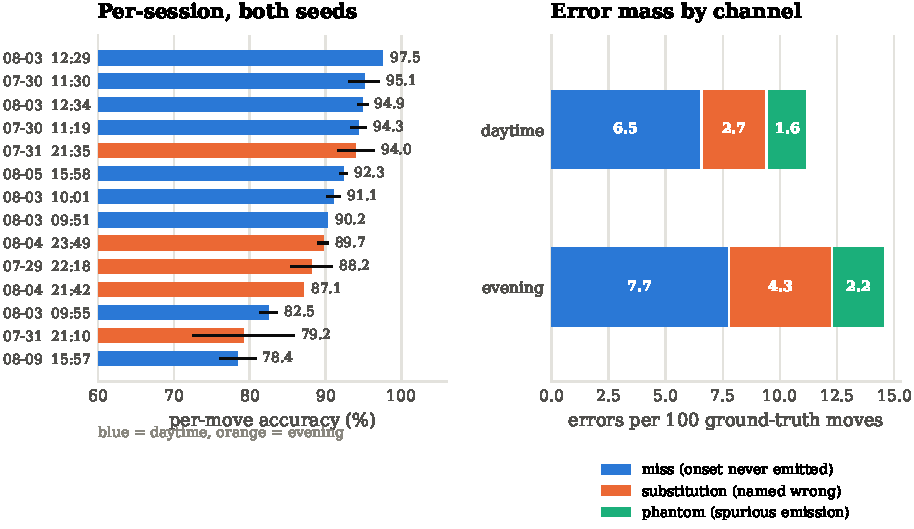
\includegraphics[width=\linewidth]{figures/fig_persession.pdf}
\caption{Left: per-session accuracy on the held-out set; bar is the two-seed
mean, black line the spread. Right: where the error mass goes. Misses
dominate in both lighting regimes.}
\label{fig:persession}
\end{figure}

\paragraph{Decoding choice.} Prefix beam search over the posteriorgram beats
best-path (greedy) decoding by \GreedyGap\ points on average --- small, but
consistent, and free.

\paragraph{Error composition.} Pooled over the holdout and both seeds:
\MissRate\ misses, \SubRate\ substitutions and \PhantomRate\ phantoms per 100
ground-truth moves. As shares of total error mass that is
\MissShare\% miss, \SubShare\% substitution, \PhantomShare\% phantom. The
implication runs through the rest of this report: \textbf{the pipeline's
dominant failure is not naming a move wrongly, it is not seeing it at all},
and the group decoder's strongest channel is the smallest one.

\subsection{How much of that number is generalisation?}
\label{sec:ladder}

\begin{figure}[t]
\centering
\begin{minipage}{0.47\linewidth}
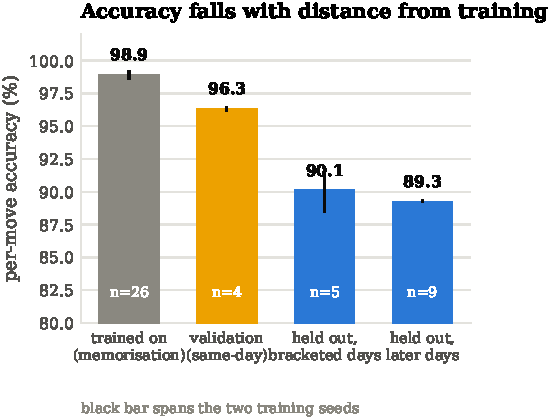
\includegraphics[width=\linewidth]{figures/fig_ladder.pdf}
\end{minipage}\hfill
\begin{minipage}{0.5\linewidth}
\small
The same weights, scored on four tiers of increasing distance from training.
The \LadderValMinusHeld-point drop from validation to genuinely-unseen
sessions is the size of the error a same-day validation split makes. Note
that ``bracketed'' days
(held out, but sandwiched between training days) score no better than
``later'' days --- so this is not primarily temporal extrapolation, it is
simply \emph{unseen session}.
\end{minipage}
\caption{Holdout proximity ladder. Bars are the two-seed mean; the black
line spans the seeds.}
\label{fig:ladder}
\end{figure}

Accuracy falls monotonically with distance from training:
\LadderTrain\% on sessions the checkpoints trained on, \LadderVal\% on the
same-day validation sessions that chose the stopping epoch, and
\LadderHeld\% on sessions never seen in any capacity --- a
\LadderTrainMinusHeld-point spread.

Two readings follow.

\begin{enumerate}[leftmargin=1.4em,itemsep=3pt]
\item \textbf{Validation MER cannot rank interventions here.} It sits
\LadderTrainMinusVal\ points below train and \LadderValMinusHeld\ above the
honest holdout, on same-day neighbours. \cref{sec:ablation} shows two interventions that validation
called flat and the holdout calls large.
\item \textbf{The repository's published numbers are optimistic, and by a
knowable amount.} Scored under this report's harness, the eight sessions the
repository calls held out give 89.9\%/92.7\% by seed; the strictly-defined
14 give \RawAllSA\%/\RawAllSB\%. The difference is small, but it is in the
direction the selection predicts, and the eight included two validation
sessions.
\end{enumerate}

\subsection{The ablation ladder}
\label{sec:ablation}

\begin{table}[t]
\centering\small
\caption{Five checkpoint generations, two seeds each, all scored on the
\emph{same} \NHoldoutSolves\ never-seen solves. ``train'' is the number of
sessions that configuration trained on.}
\label{tab:ablation}
\begin{tabular}{@{}lrrrr@{}}
\toprule
configuration & train & daytime & evening & all \\
\midrule
peak-pick (joint) & 38 & 78.2\% & 63.9\% & 73.1\% \\
CTC & 38 & 81.9\% & 61.0\% & 74.4\% \\
CTC + photo-aug & 38 & 82.6\% & 73.3\% & 79.3\% \\
CTC + photo-aug + 6 sessions & 44 & 86.0\% & 78.7\% & 83.4\% \\
CTC + photo + speed aug & 44 & 90.7\% & 87.6\% & 89.6\% \\
\bottomrule
\end{tabular}

\end{table}

\begin{figure}[t]
\centering
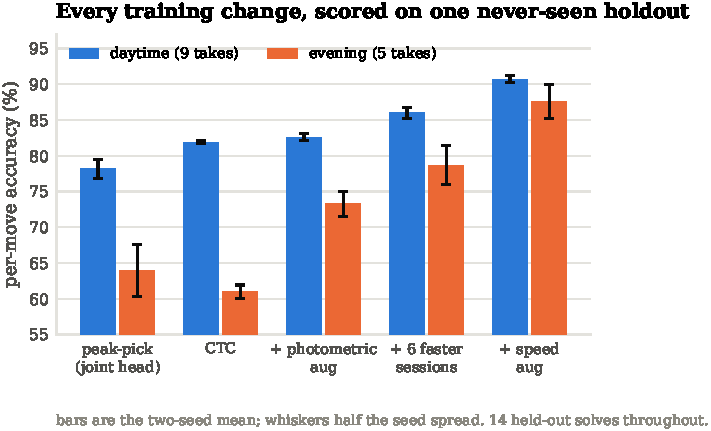
\includegraphics[width=0.92\linewidth]{figures/fig_ablation.pdf}
\caption{Each rung adds exactly one thing to the rung below it. The holdout
is intersected across all ten checkpoints, so no rung is scored on a session
any rung has seen.}
\label{fig:ablation}
\end{figure}

This is the first time these five configurations have been comparable: each
was historically evaluated on whatever holdout existed that week. Because
every rung is scored on the same \NPaired\ sessions, the rungs can be
compared \emph{pairwise}, which is far more powerful than comparing two
means:

\begin{center}\small
\begin{tabular}{@{}lrrr@{}}
\toprule
step & $\Delta$ accuracy & 95\% CI & sign test \\
\midrule
peak-picking $\to$ CTC & \DCtcVsPeak &
  [\DCtcVsPeakLo, \DCtcVsPeakHi] & $p = $ \DCtcVsPeakP \\
$+$ widened photometric augmentation & \DPhotoAug &
  [\DPhotoAugLo, \DPhotoAugHi] & $p = $ \DPhotoAugP \\
$+$ six more (faster) training sessions & \DMoreSessions &
  [\DMoreSessionsLo, \DMoreSessionsHi] & $p$ \DMoreSessionsP \\
$+$ speed augmentation & \DSpeedAug &
  [\DSpeedAugLo, \DSpeedAugHi] & $p$ \DSpeedAugP \\
\midrule
first rung $\to$ last rung & \DTotal &
  [\DTotalLo, \DTotalHi] & $p$ \DMoreSessionsP \\
\bottomrule
\end{tabular}
\end{center}

\begin{description}[leftmargin=1.2em,style=nextline,itemsep=4pt]
\item[Peak-picking $\to$ CTC: \DCtcVsPeak\ points, \emph{not significant}
($p = $ \DCtcVsPeakP, \DCtcVsPeakBetter\ sessions better,
\DCtcVsPeakWorse\ worse).] This is the project's headline architectural
change and on this holdout it cannot be distinguished from noise. What
\emph{does} change dramatically is the error composition: substitutions and
phantoms fall sharply while misses rise --- CTC trades ``fires and names it
wrong'' for ``does not fire''. Whether that is an improvement depends on the
consumer: for the group decoder it is \emph{worse}, because substitutions
are its cheap channel and misses its expensive one; for the count gate it is
roughly neutral. The defensible case for CTC is not this delta, it is that
CTC removes the constant-tuning failure mode of \cref{sec:peakpick} and that
its advantage grows with every later rung.
\item[Widened photometric augmentation: \DPhotoAug\ points, marginal
($p = $ \DPhotoAugP).] Concentrated almost entirely in the evening
(\PhotoAugEveningGain\ there, \PhotoAugDaytimeGain\ daytime), which is why
the pooled test is weak: it is a large effect on 5 of \NPaired\ sessions.
This is the synthetic substitute for evening data and within its regime it
works.
\item[Six more (faster) training sessions: \DMoreSessions\ points
($p$ \DMoreSessionsP).] Significant, and unglamorous: the corpus was stale
relative to how fast the solver had become.
\item[Speed augmentation: \DSpeedAug\ points ($p$ \DSpeedAugP),
\DSpeedAugBetter\ of \NPaired\ sessions better.] \textbf{The largest and
most significant single accuracy intervention in the project's history ---
and it was recorded as costing nothing.} It was introduced to stop the count
gate under-reading fast solves, judged on validation MER (which was flat,
correctly: the validation sessions are slow), and shipped as a neutral
change.
\end{description}

\begin{keybox}
The pattern is the result. \textbf{The two \emph{data} interventions are
significant and the two \emph{method} interventions are not} --- and both
data interventions were invisible to the validation metric used to judge
them, for the same structural reason: the validation split is
same-day-adjacent and therefore drawn from the regime that already worked. A
holdout is not a formality; on this corpus it is the only instrument that
can see the interventions that matter.
\end{keybox}

Total across the ladder: \DTotal\ points [\DTotalLo, \DTotalHi] on the same
never-seen sessions.

\subsection{Error analysis}
\label{sec:erroranalysis}

\begin{figure}[t]
\centering
\begin{minipage}{0.47\linewidth}
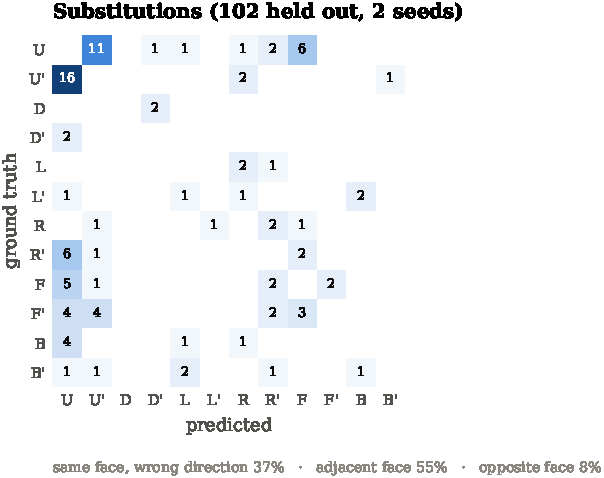
\includegraphics[width=\linewidth]{figures/fig_confusion.pdf}
\end{minipage}\hfill
\begin{minipage}{0.47\linewidth}
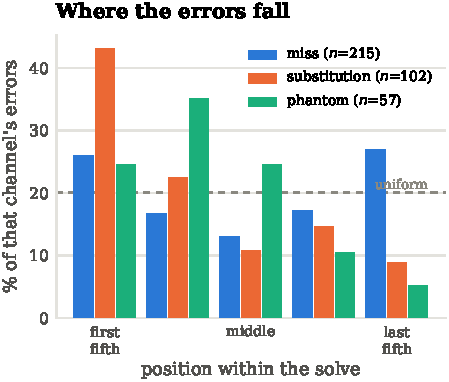
\includegraphics[width=\linewidth]{figures/fig_errpos.pdf}
\end{minipage}
\caption{Left: the \NSubTotal\ substitutions on the holdout, both seeds.
Right: where each error channel falls within a solve.}
\label{fig:erroranalysis}
\end{figure}

\paragraph{Substitutions are mostly adjacent-face, not direction errors.}
\SubAdjacent\% name a face adjacent to the true one, \SubInverse\% get the
face right and the direction wrong, \SubOpposite\% name the opposite face.
This settles a question the project re-litigated repeatedly: on
\emph{in-distribution} data the residual error is direction confusion (the
hard case that survives when everything else works), but in the live long-solve
regime it is a more basic wrong-face error. The held-out measurement here
agrees with the live regime, which is the one that matters. An architecture
change that models time more richly targets the \SubInverse\% channel, not
the \SubAdjacent\% one.

\paragraph{There is a prediction bias toward the U layer.}
\PredUShare\% of all substitution \emph{predictions} are \wca{U} or \wca{U'},
against $\tfrac{2}{12}=17$\% under a uniform prior. The U layer is the most
frequent class in CFOP by a wide margin, and the model falls back on it when
unsure --- classic prior collapse, and a candidate for class-balanced
training or a logit prior correction. Not yet tried.

\paragraph{Errors are strongly non-uniform through a solve, and each channel
has its own shape.} \SubFirstFifth\% of substitutions fall in the first
fifth of the solve against \SubLastFifth\% in the last --- more than double
the uniform 20\%. Phantoms are similarly front-loaded
(\PhanFirstFifth\% vs \PhanLastFifth\%). Misses are the opposite shape:
roughly U-distributed, \MissFirstFifth\% at the start and
\MissLastFifth\% at the end with a trough in the middle.

The interpretation is CFOP's phase structure. The opening --- inspection,
cross, first F2L pair --- is where the cube is rotated and regripped most,
which is precisely the motion that looks like a turn without being one; that
produces both wrong names and spurious detections. The last fifth is the
last layer: fast, memorised, heavily crowded algorithm execution, where the
failure is not seeing turns at all.

This matters for the decoder. Its endpoint constraint is weakest exactly
where substitutions cluster (the beginning, dozens of moves from the only
anchor) and strongest where misses cluster (the end) --- but misses are the
channel it cannot cheaply repair. The two distributions are almost
maximally unhelpful to it.

\subsection{The truth frame is worth measuring}
\label{sec:frame-result}

Scoring the identical predictions against cube-frame truth (what the smart
cube reports, and what every harness in the repository still uses) versus
camera-frame truth (what a vision model can possibly predict,
\cref{sec:labelframe}):

\begin{center}\small
\begin{tabular}{@{}lrr@{}}
\toprule
scored over & cube-frame truth & camera-frame truth \\
\midrule
the three slice-bearing held-out sessions & \FrameCubeSlice\% &
\FrameCamSlice\% \\
the whole held-out set & \FrameCubeAll\% & \FrameCamAll\% \\
\bottomrule
\end{tabular}
\end{center}

\FrameGainSlice\ points where it applies, \FrameGainAll\ diluted over the
holdout. Small --- but it is a systematic bias against the model, it is free
to fix, and it is exactly the kind of thing that erodes confidence in
everything else in a paper when a reviewer finds it.

\subsection{The group decode and the falsifiability sweep}
\label{sec:decode-results}
\label{sec:falsifiability}

\begin{table}[t]
\centering\small
\caption{Group-theoretic decode, both seeds, on every held-out free solve.
$\Delta$ is post-decode minus raw. ``decoys accepted'' counts, out of eight
per session (four false claims $\times$ two seeds), how many wrong start
states the decoder found a valid story for. $\dagger$ marks sessions
containing a middle slice, where the decoder's cube-frame model and the
recogniser's camera-frame output are known to disagree
(\cref{sec:labelframe}).}
\label{tab:decode}
\begin{tabular}{@{}lrrrccc@{}}
\toprule
session & raw & post & $\Delta$ & verified & exact & decoys accepted \\
\midrule
07-29\,22:18$^{\dagger}$ & 86.8\% & 85.9\% & -1.0 & 0/2 & 0/2 & 0/8 \\
07-30\,11:19 & 94.3\% & 94.8\% & +0.5 & 0/2 & 0/2 & 0/8 \\
07-30\,11:30$^{\dagger}$ & 93.6\% & 93.6\% & +0.0 & 0/2 & 0/2 & 0/8 \\
07-31\,21:10 & 79.2\% & 79.2\% & +0.0 & 0/2 & 0/2 & 0/8 \\
07-31\,21:35 & 94.0\% & 93.1\% & -0.9 & 0/2 & 0/2 & 0/8 \\
08-03\,09:51 & 90.2\% & 89.6\% & -0.6 & 0/2 & 0/2 & 0/8 \\
08-03\,09:55$^{\dagger}$ & 78.9\% & 79.3\% & +0.4 & 0/2 & 0/2 & 0/8 \\
08-03\,10:01 & 91.1\% & 91.1\% & +0.0 & 0/2 & 0/2 & 0/8 \\
08-03\,12:29 & 97.5\% & 97.5\% & +0.0 & 0/2 & 0/2 & 0/8 \\
08-03\,12:34 & 94.9\% & 94.9\% & +0.0 & 0/2 & 0/2 & 0/8 \\
08-04\,21:42 & 87.1\% & 87.1\% & +0.0 & 0/2 & 0/2 & 0/8 \\
08-04\,23:49 & 89.7\% & 89.7\% & +0.0 & 0/2 & 0/2 & 0/8 \\
08-05\,15:58 & 92.3\% & 92.7\% & +0.4 & 0/2 & 0/2 & 0/8 \\
08-09\,15:57 & 78.4\% & 78.4\% & +0.0 & 0/2 & 0/2 & 0/8 \\
\bottomrule
\end{tabular}

\end{table}

\begin{figure}[t]
\centering
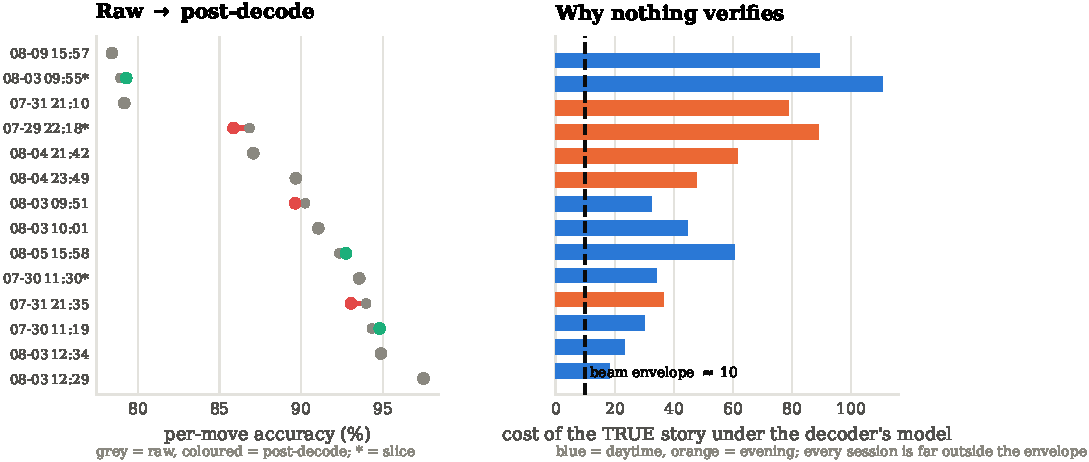
\includegraphics[width=\linewidth]{figures/fig_decode.pdf}
\caption{Left: what the group decode does to each session's accuracy.
Right: the falsifiability sweep --- the fraction of claims the decoder found
a solving story for, when the claim is true and when it is deliberately
wrong by 1, 2 or 4 quarter turns or entirely fabricated.}
\label{fig:decode}
\end{figure}

\begin{figure}[t]
\centering
\begin{minipage}{0.46\linewidth}
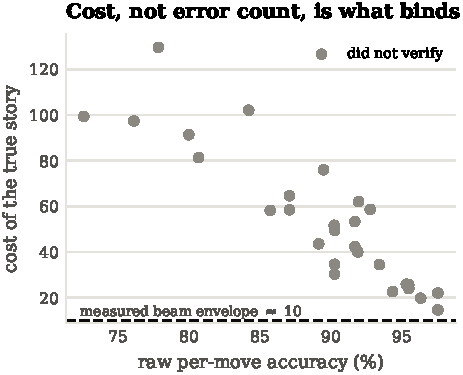
\includegraphics[width=\linewidth]{figures/fig_cliff.pdf}
\end{minipage}\hfill
\begin{minipage}{0.5\linewidth}\small
The decode's binding constraint is the \emph{cost} of the true story under
the model, not the number of errors in it. A story costing ${\sim}6$ survives
90 onsets at the deployed beam; one costing ${\sim}10$ does not, and every
insertion is a flat 4.0. On this holdout the cheapest true story costs
\MinGtPathCost\ and the median costs \MedGtPathCost\ --- every session is
outside the envelope, which is why the scatter has no verified points in it
at all.
\end{minipage}
\caption{Why the decode is all-or-nothing, and why on this holdout it is
uniformly ``nothing''.}
\label{fig:cliff}
\end{figure}

\textbf{The decode contributes nothing measurable on this holdout.} On the
\DecodeNonSliceN\ slice-free held-out solves it moves per-move accuracy from
\DecodeRaw\% to \DecodePost\% --- \DecodeGain\ points --- and it verifies
\DecodeVerified\ of \DecodeTrials\ session-seed pairs. Twenty of the 28
session-seed pairs are unchanged to three decimal places; of the eight that
move, four improve and four get \emph{worse}.

That is a substantially weaker result than the repository's ${\sim}+1.2$
points daytime, and the difference is not a contradiction --- it is the
holdout. The older figure was measured on a set whose sessions included
several with true-story costs near the beam's envelope; this holdout has
none. Which is exactly the prediction \cref{sec:decode-limits} makes: the
decode is worth about a point where it closes and nothing where it does not,
so a holdout two points harder collapses its contribution to zero.

\paragraph{The mechanism, restated with the numbers.} The endpoint
constraint is global and terminal. The cheapest true story on this holdout
costs \MinGtPathCost\ against an envelope of ${\sim}10$, and the median costs
\MedGtPathCost. At \MissShare\% miss-dominated error, each missing move
charges a flat $C_{\rm ins} = 4.0$ with no posterior evidence to offset it,
so a session with even five misses is already outside the envelope before
any naming error is counted. The sessions that most need repair are
precisely the ones whose repair is unaffordable.

\paragraph{Beam budget.} These runs use the deployed first-pass beam of
4000 without the production retry at $4\times$. That is a compute
concession, and it is checkable rather than assumed: a wider beam searches
the same cost landscape, and with the cheapest true story at
\MinGtPathCost\ there is nothing within the envelope for it to find. It
could in principle change a \emph{best-effort} story slightly; that is
untested here and is the one caveat on the \DecodeGain-point figure.

\paragraph{Slice sessions fail structurally, not statistically.} The
$\dagger$ sessions carry the highest costs relative to their raw accuracy,
because the model emits camera-frame move names into a decoder whose cube
model is centre-relative. This is a known, unfixed defect; the machinery to
handle it (persistent orientation state in the beam) exists and is disabled
on a premise --- ``the recorded sessions hold one orientation throughout'' ---
that these sessions falsify.

\paragraph{Falsifiability, and why this run cannot speak to it.}
\DecoyAccepted\ of \DecoyTried\ deliberately false claims were accepted.
\textbf{That is not a security result and must not be reported as one},
because the same decoder also rejected all \DecodeTrials\ \emph{true}
claims. A verifier that rejects everything has perfect specificity and zero
sensitivity; the sweep is uninformative when the true-positive rate is zero.

Two things do survive from it. First, the operational statement: at the
deployed beam nothing spurious was accepted. Second, and more usefully, the
constructive bound of \cref{eq:decoybound} still applies --- a valid story
for a $d$-move-off claim provably exists at $c(W) + 4d$, so any rejection
here is the search failing to find a story that is known to be there, not
the cost model ruling it out. A meaningful falsifiability measurement
requires sessions whose true claims verify, and this holdout has none. That
is a reason to record easier sessions for that specific test, not a reason
to quote 0/\DecoyTried.

\subsection{The count gate}
\label{sec:anticheat-results}

\begin{figure}[t]
\centering
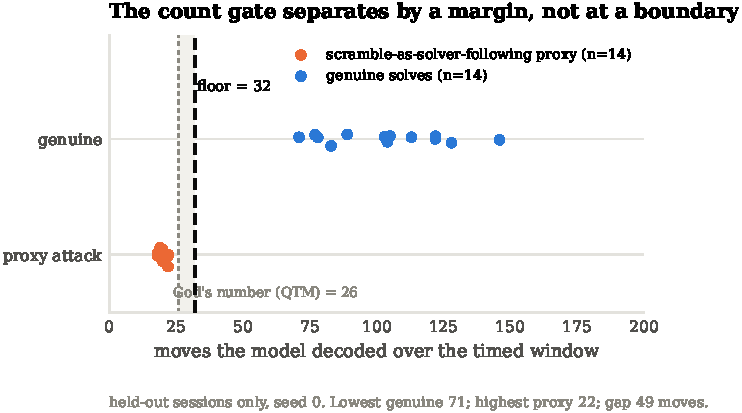
\includegraphics[width=0.92\linewidth]{figures/fig_anticheat.pdf}
\caption{Decoded move count on held-out sessions. Genuine solves and
scramble-as-solver-following proxies do not merely fall on opposite sides of
the threshold --- they are separated by \ACGapSA\ moves with the threshold
inside the gap.}
\label{fig:anticheat}
\end{figure}

On the strict holdout: \ACVerifiedSA/\ACSolves\ and
\ACVerifiedSB/\ACSolves\ genuine solves verified with zero false
disqualifications on either seed, and \ACCaughtSA/\ACProxies\ and
\ACCaughtSB/\ACProxies\ proxy attacks caught on either seed. The lowest
genuine solve reads \ACLowestLegit\ moves; the highest proxy reads
\ACHighestProxy; the floor of 32 sits inside a gap of
\ACGapSA--\ACGapSB moves. Minimum headroom above the floor on a genuine
solve is \ACHeadroomSA/\ACHeadroomSB moves.

This is the strongest result in the report, and the reason is structural
rather than statistical: the gate asks the model a question it is good at
(how many events) rather than one it is bad at (which event), and the
quantity it thresholds is bounded by a theorem rather than by a fit.
\Cref{sec:verification} states the one physical attack that survives it.

\begin{keybox}
\textbf{The catch side is a proxy.} A prescribed scramble is structurally
identical to solver-following --- a short machine-generated sequence executed
by hand on camera --- and it is uncontaminated precisely because it was
recorded for another purpose. But nobody has attacked this system. The catch
rate measures a separation, not a defeat.
\end{keybox}

\subsection{Regime analysis, and why the analysis stops here}
\label{sec:regime}

Evening sessions are worse than daytime by
\EveningGapPts\ points on average. Adding a lamp to the same room, same
evening, same cube recovered most of that in a controlled test --- so
lighting is causal, not correlational. The corpus is 87\% daytime, which is
the textbook data-hole signature.

Beyond that, attribution fails, and the failure is worth recording because
the next person will otherwise repeat it. Four candidate mechanisms for the
$16\times$ per-session miss-rate spread were tested against the held-out
misses: half turns ($p = 0.105$, ceiling 0.61 points), onset crowding
(median 3.0 frames to nearest neighbour for missed onsets vs 4.0 for found,
$p = 0.21$), sensor quiet-frame noise floor (a \emph{perfect} 4-vs-4 split
with $r = -0.72$), and posterior separability (the metric produced
out-of-range values and tested nothing).

The third looked decisive and does not survive two checks. The proposed
mechanism runs backwards --- median onset confidence \emph{at true onsets} is
higher in the failing sessions (0.729) than the passing ones (0.656), so
whatever is happening is not signal suppression. And it is a six-variable
search over eight sessions: a random variable splits 4-worst from 4-best
perfectly with probability $1/\binom{8}{4} = 1.4\%$, so across six variables
${\sim}8\%$ of the time by chance. Two other variables with no story at all
separated nearly as well.

\begin{keybox}
\textbf{The binding constraint on this project is the number of held-out
sessions, not the number of hypotheses.} At $n$ in the low tens, analysis
cannot distinguish a real regime axis from a lucky one, and more variables
will keep producing spurious separations. This report doubles $n$ from 8 to
\NHoldoutSolves\ and that is still not enough to carry a multiple-comparisons
correction. Record more sessions first; attribute after.
\end{keybox}

\section{Discussion}
\label{sec:discussion}

\subsection{What the numbers actually support}

Three claims survive the holdout discipline of \cref{sec:holdout-hygiene}.

\begin{enumerate}[leftmargin=1.4em,itemsep=3pt]
\item \textbf{A small CTC video model reads a human speedsolve at
\CIDayMean\% [\CIDayLo, \CIDayHi] per-move accuracy in reasonable light}, on
\NHoldoutSolves\ solves it has never seen, at a median
\MedianTPS\,turns/s with \CrowdedPctHoldout\% of turn pairs within two frames.
The structural CTC ceiling for this corpus is \CTCCeilingHoldout\%, so about
\RemainingGap\ points of the remaining gap are addressable in principle.
\item \textbf{Move \emph{counting} separates a genuine solve from a
solver-following proxy by tens of moves}, with zero false disqualifications
across \ACSolves\ held-out solves on both seeds. Unlike everything else here,
the quantity being thresholded is bounded by a theorem.
\item \textbf{Held-out session count, not model capacity, is the binding
constraint.} The same weights score above 97\% on one held-out session and
below 79\% on another; capacity limits do not look like that. Every
model-side intervention on record --- encoding rework, optical flow, anchor
selection, per-frame noise --- measures flat, while every data-side one
measures large (\cref{sec:ablation}).
\end{enumerate}

And one claim that does \emph{not} survive:

\begin{keybox}
\textbf{The group-theoretic decode does not work at this error rate.} It is
worth \DecodeGain\ points on the held-out set and verifies
\DecodeVerified/\DecodeTrials. This is the most interesting result in the
report, because the decode is the conceptually strongest part of the design
--- the output space really is a group, both endpoints really are known, and
the constraint really is exact. It fails anyway, for a reason that has
nothing to do with group theory: the constraint arrives \emph{once}, at the
end, and the cheapest true story on this holdout is already
\MinGtPathCost\ against an envelope of ${\sim}10$. Constraint density, not
constraint strength, is the quantity that matters.
\end{keybox}

\subsection{The catalogue of negative results}
\label{sec:negatives}

These are more useful than the positive results for anyone deciding what to
try next, and they are collected here because each one was measured rather
than reasoned about.

\begin{center}\small
\begin{tabular}{@{}p{5.4cm}p{9.6cm}@{}}
\toprule
\textbf{Intervention} & \textbf{Measured outcome} \\
\midrule
Optical flow (RAFT and Farneback) as model input
  & Significantly \emph{worse} than raw appearance ($p \le 2\times10^{-3}$;
    54.4\% vs 70.4\%). Clean motion is not what the model wants; appearance
    beats it. \\
Richer temporal encodings (3-channel temporal colour vs 12-channel diff
stack)
  & Tie. The seed spread exceeded the effect. \\
An explicit onset-count head (predicting 0/1/2+ onsets per bin) to fix
crowding
  & Failed on premise: only 1 of 9 held-out misses was crowding-caused. \\
Forward algorithm prior (recognise a last-layer algorithm, insert it into
the beam)
  & The gate never admits a hypothesis: a median 60\% of the true story's
    cost is spent before the last layer begins. Inert. \\
Backward algorithm peel with a trust threshold
  & Fails its own gate: $-0.6$ points daytime. Identification confidence says
    a peeled span is probably the right word; it does not say that using it
    beats what the plain decode already had. \\
Adding textbook OLL/PLL algorithms to the library
  & Structurally wrong: the matcher scores the \emph{executed word}, not the
    resulting permutation, so textbook entries add words this solver never
    performs. The library is user-specific by construction. \\
Statistical lighting gates from image statistics
  & Anti-correlated with the failure they were meant to predict. The clock is
    the only working predictor. \\
Pixel-level transforms to close the evening gap (noise injection to restore
the diff floor, exposure/colour/crop matching)
  & Flat across every setting tried. The mechanism is not isolated, so a
    targeted transform is aimed at a guess. \\
Anchor-selection improvements in the group decode
  & Oracle ceiling measured at $+0.65$ points; six of eight daytime sessions
    have \emph{exactly zero} anchor headroom. Built anyway, measured $-0.6$.\\
Appearance-based swap detection
  & Dead: a legit solve \emph{completing} is the largest appearance jump in a
    session. \\
Half-turns as their own class (\wca{R2})
  & Worth $\le 0.61$ points ($p = 0.105$), requires relabelling 40\% of the
    corpus, and silently breaks the QTM anticheat calibration. \\
\bottomrule
\end{tabular}
\end{center}

\noindent The pattern is unmistakable: \textbf{every decoder-side and
representation-side lever has measured flat, and every data-side lever has
measured large.} That is what a coverage-limited system looks like.

\subsection{Methodological lessons}

These generalise past this project and are the part of this report most
worth keeping.

\begin{description}[leftmargin=1.2em,style=nextline,itemsep=4pt]
\item[A validation split adjacent in time to training is not a holdout.]
It is 6.2 points optimistic here, and --- worse --- it is optimistic
\emph{selectively}: it is blind to exactly the interventions that address
the regimes it does not contain. Two of the four ablation rungs in
\cref{sec:ablation} were called flat by validation and large by the holdout.
\item[When a retrain fixes a regime, find out what else changed.] The
crop-regime incident (\cref{sec:preproc}) attributed a 29-point improvement
to ``more live training data'' when the real cause was that the evaluation
had been comparing full-frame-trained weights against cropped test input.
The same weights, re-scored consistently, went from 61.5\% to 90.6\% with no
retraining at all.
\item[A passing consistency check is evidence only about what it can see.]
The session checker validated the cube-frame product of the labels and was
structurally blind to camera-frame drift, because its cube model has no
centres (\cref{sec:labelframe}). It reported 16/16 for weeks.
\item[Quantify a defect before treating it as a lever.] Window-anchor
mismatch was real, measurable, and worth 0.3 points. Crowding was real and
worth 1 of 9 misses. A defect being genuine says nothing about its size.
\item[State the constructive bound alongside the empirical rejection.] The
decoy sweep rejects near-miss claims operationally, and
\cref{eq:decoybound} proves a cheap wrong story exists anyway. Reporting only
the first would be the easiest available way to oversell this system.
\item[Report per-session floors, not just means.] A user experiences their
own solve. A mean of \RawDayMean\% with a floor of \RawMinSA\% is a different
product from a mean of \RawDayMean\% with a floor of 88\%.
\end{description}

\subsection{Limitations}
\label{sec:limitations}

\begin{itemize}[leftmargin=1.3em,itemsep=3pt]
\item \textbf{$n=1$ solver.} One person, one cube, two rooms, three weeks.
Nothing here speaks to cross-person generalisation, and the measured
cross-\emph{day} degradation within one person is a lower bound on it.
\item \textbf{The training signal requires hardware most users do not own.}
Every label came from a Bluetooth cube. Scaling the corpus beyond this one
solver requires either more smart-cube owners or a labelling path that does
not need one --- a human review tool exists and has never been used at scale.
\item \textbf{No external baseline.} There is no published system, dataset,
or prior number to compare against. Every comparison in this report is
internal, which means it can establish that a change helps but not that the
absolute level is good.
\item \textbf{Non-causal model.} Frame $t$ sees one second of future. Fine
for buffer-then-analyse; a live streaming product would need causal padding
and would pay for it at the leading edge.
\item \textbf{The decoder and the recogniser disagree about reference frame}
on slice-bearing sessions (\cref{sec:decode-results}). Known, unfixed.
\item \textbf{The evaluation ground truth is itself a model of the world}
--- the smart cube's move stream, which has 30\,ms tick collisions
(${\sim}10$\% of moves), up to one frame of alignment noise, and an
unreliable state query. Ground truth here is good, not perfect.
\item \textbf{Adversarial evaluation is entirely synthetic.} No recorded
attack of the one shape that survives the count gate exists.
\end{itemize}

\section{What would have to be true for this to be a paper}
\label{sec:gap}

This section is the point of the document. The measurements above are real,
but a venue would reject this work as written, and it is worth being precise
about why --- most of the objections are about evidence, not method, and
several are cheap to fix.

\subsection{Blocking gaps}

\paragraph{G1. The corpus is one person.} Every reviewer's first question
will be whether the model has learned ``how a cube turns'' or ``how
\emph{this} person's hands look''. \cref{sec:ladder} shows a
\LadderTrainMinusHeld-point degradation across \emph{days} within one
person; across people it will be larger, and the direction is not in doubt.

\emph{What fixes it:} 5--10 additional solvers, ${\sim}10$ solves each,
different cubes, different rooms. With BLE labels that is a hardware
constraint; without them it needs the human-review labelling path. A
leave-one-solver-out protocol then becomes possible, and that --- not the
number in \cref{tab:main} --- is the result a paper reports.

\paragraph{G2. There is no baseline.} Every number here is internal.
\cref{sec:ablation} establishes that the pipeline improved, not that it is
good.

\emph{What fixes it:} at minimum (a) a classical-CV baseline --- frame
differencing plus optical-flow direction voting --- so the learned model has
a floor to beat; (b) a strong generic video-classification baseline, e.g.\ a
small video transformer or an inflated 3-D CNN on the same clips, to show the
domain-specific architecture earns its specificity; (c) an off-the-shelf
CTC-over-frozen-features baseline. All three are days of work, not weeks,
and the third is the one most likely to embarrass the current design.

\paragraph{G3. The evaluation set is too small to attribute anything.}
\cref{sec:regime} documents an honest attempt at attribution collapsing
under multiple comparisons at $n=8$; this report's $n=\NHoldoutSolves$ does
not fix it. Statements of the form ``lighting causes the gap'' currently
rest on a single controlled lamp intervention.

\emph{What fixes it:} 40--60 held-out solves stratified by lighting, speed
and solver, which makes a two-way analysis possible and lets a
Bonferroni-corrected regime claim survive.

\paragraph{G4. The adversarial evaluation contains no adversary.}
\cref{sec:anticheat-results}'s catch rate is a proxy. Any security venue
rejects on this alone.

\emph{What fixes it:} record the attacks. Specifically the one that survives
the count gate --- plausible moves without solving, then a swap, including
the table-edge variant --- plus genuine solver-following, plus
timer-stop-then-solve. Twenty of each is enough to state a ROC rather than a
count.

\subsection{Fixable weaknesses that would draw fire}

\begin{description}[leftmargin=1.2em,style=nextline,itemsep=4pt]
\item[The intervals are wide, and two headline claims do not survive them.]
This draft \emph{does} bootstrap over sessions and test the ablation
pairwise (\cref{sec:ablation}), which was originally on this list --- and
doing it changed the story. The CTC migration, the project's headline
architectural change, comes out at \DCtcVsPeak\ points with a CI spanning
zero. Photometric augmentation is marginal. Only the two data interventions
survive. Any future claim needs the same treatment \emph{before} it is
written down, not after.
\item[The regime split is not statistically separated.] Daytime
\CIDayMean\% [\CIDayLo, \CIDayHi] and evening \CIEveMean\%
[\CIEveLo, \CIEveHi] overlap substantially at $n=9$ and $n=5$. The lamp
intervention is stronger evidence for the causal claim than the split is,
and it is a single controlled comparison.
\item[The frame-reference defect is live in the repository.] Every harness
except this report's scores against cube-frame truth
(\cref{sec:labelframe}). Small, but it is the kind of thing a careful
reviewer finds and then distrusts everything else.
\item[The decoder's cost constants are unjustified.] $C_{\rm del}=2.6$,
$C_{\rm ins}=4.0$, $\lambda_i=0.20$, $\lambda_u=0.04$ are described as
$-\log$ of measured odds but were never re-derived after the recogniser
changed twice. They should be re-fit on held-out sessions, or at least a
sensitivity sweep reported.
\item[The prediction bias toward the U layer (\cref{sec:erroranalysis}) is
unaddressed.] \PredUShare\% of substitution predictions are \wca{U}/\wca{U'}.
Class-balanced loss or a logit prior correction is a one-line experiment.
\item[The spatial average pool discards where the motion was.] The single
most obvious architectural question --- does a model that retains coarse
spatial structure name faces better? --- has never been asked, and
\SubAdjacent\% of substitutions are wrong-face errors.
\item[The abstain path is untested end to end.] The count gate has three
tiers, and no held-out session has ever triggered \texttt{REVIEW}. That means
the abstain logic is unexercised, not that it is reliable.
\item[The post-stop phantom rate is extrapolated.] Calibrated on 1--3\,s
session tails and applied to a window of tens of seconds.
\end{description}

\subsection{Things that would make it a genuinely interesting paper}

Not required, but these are what would give it a thesis rather than a
system description.

\begin{enumerate}[leftmargin=1.4em,itemsep=4pt]
\item \textbf{``Structured output as a substitute for accuracy.''} The
sharpest idea in the system is that a hard algebraic constraint on the output
space converts an impossible sequence-level problem into a tractable one ---
and the honest finding (\cref{sec:decode-results}) is that at this error
rate it does \emph{nothing at all}, for a specific and generalisable reason:
the constraint is terminal, so it discriminates nothing until the end.
Quantifying the relationship between \emph{constraint density} and recovery
--- by artificially injecting mid-solve state observations at varying spacing
and measuring where recovery switches on --- would turn a null result into a
finding. It is a clean, cheap experiment, it needs no new data, the current
0/\DecodeTrials\ is the $d=\infty$ endpoint of its own curve, and the result
would transfer to any constrained-decoding setting. \textbf{This is the one
experiment I would actually run next.}
\item \textbf{``Counting is robust where identification is not.''} The
anticheat result is the strongest here, and its structure is general: when
identification is unreliable, find a decision that depends only on a
statistic the model estimates well, and bound that statistic with a theorem
rather than a fit. The verification cliff at ${\sim}98\%$ versus the count
gate's tens-of-moves margin is a crisp illustration.
\item \textbf{An honest negative-result paper on the evaluation trap.}
\cref{sec:ablation}'s finding --- that the validation split was structurally
blind to the two largest interventions, and that both were shipped or nearly
discarded on its say-so --- is a better contribution than any accuracy
number in this document.
\end{enumerate}

\subsection{The order I would do these in}

\begin{enumerate}[leftmargin=1.4em,itemsep=2pt]
\item Fix the frame-reference defect in the repository's harnesses, and
enable persistent orientation in the group decoder (one day).
\item The constraint-density experiment (item 1 above) --- no new data, and
it is the potential thesis.
\item Recruit 5--10 solvers. Everything else is gated on this.
\item Record the attacks.
\item Baselines.
\end{enumerate}

\section{Conclusion}
\label{sec:conclusion}

A \NParams-parameter convolutional model trained with a CTC objective reads
a human speedsolve from a webcam at \CIDayMean\% [\CIDayLo, \CIDayHi]
per-move accuracy in reasonable light and \CIEveMean\%
[\CIEveLo, \CIEveHi] in poor light, measured on
\NHoldoutSolves\ solves and \NHoldoutMoves\ turns that no evaluated
checkpoint has seen in training or in validation. A group-theoretic beam
search over edits then attempts to repair the transcript against the known
scramble and the solved end state --- and, on this holdout, achieves
\DecodeGain\ points and \DecodeVerified\ verifications out of
\DecodeTrials. A move-count gate --- thresholding a quantity bounded by
God's number rather than by a fit --- separates genuine solves from
solver-following proxies by tens of moves with no false disqualifications.

The two things worth carrying away are both negative, and both are about
measurement rather than method.

The first is that the constraint which makes this problem tractable in
principle --- the output space is a group and both endpoints are known ---
buys \emph{nothing measurable} at this error rate, and the reason
generalises. The constraint is \emph{terminal}: it discriminates nothing
until the last move, so it repairs sessions that were nearly right already
and abandons the ones that were not. On a holdout with no nearly-right
sessions it abandons all of them. Constraint \emph{density}, not constraint
strength, is what a decoder can use, and that is a measurable, testable
claim this corpus is well set up to answer (\cref{sec:gap}).

The second is that the validation split used to steer this project was
structurally incapable of ranking its two largest interventions, because it
was drawn from the regime that already worked. The ablation in
\cref{sec:ablation} exists only because the holdout was re-derived from the
checkpoints themselves and doubled in size; on the old split, speed
augmentation looks free, and on this one it is the largest and most
significant change on record. The same measurement, run the same way, also
says the headline architectural change --- migrating to CTC --- cannot be
distinguished from noise. Both of those are only visible from an honest
holdout with intervals attached. A holdout is not paperwork; it is the only
instrument in the building that can see the things that matter.

\appendix
\section{Notation and glossary}
\label{app:notation}

\begin{center}\small
\begin{tabular}{@{}lp{11.4cm}@{}}
\toprule
\textbf{Term} & \textbf{Meaning here} \\
\midrule
onset & the instant a turn begins; the event the model must place \\
turn / move & one quarter turn, one of the 12 alphabet symbols \\
QTM / HTM & quarter- / half-turn metric. This system is entirely QTM \\
take & one recording; a \emph{scramble} take or a \emph{solve} take \\
session & synonym for take; the unit of the holdout split \\
posteriorgram & the $T\times13$ matrix of per-frame class posteriors \\
miss & a true move the decoder never emitted (recall failure) \\
phantom & an emitted move that was not performed (precision failure) \\
substitution & a move emitted at roughly the right place, named wrong \\
MER & move error rate: Levenshtein distance $\div$ true length \\
per-move accuracy & aligned matches $\div$ true length. Does not charge
  phantoms; MER does \\
raw / post-decode & before / after the group-theoretic repair \\
verified & the group decode found a story reaching solved (accuracy tier),
  \emph{or} the count gate returned \texttt{VERIFIED} (legitimacy tier) ---
  the two are unrelated and the text always says which \\
decoy & a deliberately false claim used to test the verifier \\
bracketed / after & held-out days sandwiched between training days, versus
  strictly later than the last one \\
\bottomrule
\end{tabular}
\end{center}

\section{Reproducing every number}
\label{app:repro}

\paragraph{Environment.} Windows 11, Python 3.13, PyTorch 2.13 + CUDA 13,
NVIDIA RTX 5070 Ti Laptop, OpenCV 5.0 (contrib build --- the base package
lacks the CSRT tracker and its absence degrades detection silently).

\paragraph{Order.} Scripts live in \file{paper/scripts/} and are run from
inside \file{ble/move\_detector/}, matching the repository's convention that
scripts resolve their models and data by bare relative name.

\begin{verbatim}
cd ble
python backfill_camera_frame.py --sessions training_data/solve_*/
cd move_detector
python prepare_data.py --color --sessions ../training_data/solve_<new>/

python ../../paper/scripts/m1_recognition.py   # raw CTC + posteriorgram cache
python ../../paper/scripts/m4_ablation.py      # the five-rung ladder
python ../../paper/scripts/m5_diagnostics.py   # ladder, frame, confusion
python anticheat_gate.py score --ctc checkpoints/move_ctc_spd_s0.pt
python anticheat_gate.py score --ctc checkpoints/move_ctc_spd_s1.pt
python ../../paper/scripts/m2_decode.py --only move_ctc_spd_s0 \
       --out m2_decode_s0.json          # slow; run the two seeds in parallel
python ../../paper/scripts/m2_decode.py --only move_ctc_spd_s1 \
       --out m2_decode_s1.json

python ../../paper/scripts/mknumbers.py        # -> data/numbers.tex, tables
python ../../paper/scripts/f1_data_and_model.py
python ../../paper/scripts/f2_results.py
python ../../paper/scripts/f3_decode.py
\end{verbatim}

\paragraph{The provenance guard.} \file{paper/scripts/common.py} derives the
holdout from each checkpoint's own recorded
\texttt{train\_session\_names} and \texttt{val\_session\_names}, intersected
across every checkpoint being compared. No script in this report accepts a
hand-written session list. If a checkpoint predates the recording of those
fields, it cannot be scored at all rather than being scored on a guess.

\paragraph{Cost.} Preprocessing 18 sessions: ${\sim}6$ minutes.
Recognition sweeps: ${\sim}20$ minutes. Ablation ladder (10 checkpoints
$\times$ 14 sessions): ${\sim}25$ minutes. The group decode dominates
everything --- roughly 45\,s per decode at beam 4000 on a 130-onset session,
and each session costs one base decode, possibly a retry at beam 16000, and
four decoys.

\section{Per-session detail}
\label{app:persession}

\begin{table}[h]
\centering\small
\caption{Every held-out session, seed 0, raw CTC with prefix-beam decoding.}
\label{tab:persession}
\begin{tabular}{@{}lrrrrrrr@{}}
\toprule
session & regime & turns & turns/s & acc. & MER & miss & sub / phan \\
\midrule
07-29\,22:18 scr. & eve & 20 & 0.79 & 100.0\% & 5.0\% & 0 & 0 / 1 \\
07-29\,22:18 solve & eve & 152 & 3.08 & 85.5\% & 18.4\% & 10 & 12 / 6 \\
07-30\,11:19 scr. & day & 20 & 0.79 & 95.0\% & 5.0\% & 1 & 0 / 0 \\
07-30\,11:19 solve & day & 106 & 2.23 & 95.3\% & 6.6\% & 4 & 1 / 2 \\
07-30\,11:30 scr. & day & 20 & 0.65 & 100.0\% & 0.0\% & 0 & 0 / 0 \\
07-30\,11:30 solve & day & 132 & 2.72 & 97.0\% & 3.8\% & 3 & 1 / 1 \\
07-31\,21:10 scr. & eve & 20 & 0.76 & 100.0\% & 0.0\% & 0 & 0 / 0 \\
07-31\,21:10 solve & eve & 84 & 2.55 & 72.6\% & 27.4\% & 12 & 11 / 0 \\
07-31\,21:35 scr. & eve & 20 & 0.59 & 95.0\% & 10.0\% & 0 & 1 / 1 \\
07-31\,21:35 solve & eve & 108 & 2.88 & 91.7\% & 12.0\% & 7 & 2 / 4 \\
08-03\,09:51 scr. & day & 22 & 0.67 & 100.0\% & 0.0\% & 0 & 0 / 0 \\
08-03\,09:51 solve & day & 82 & 2.58 & 90.2\% & 11.0\% & 5 & 3 / 1 \\
08-03\,09:55 scr. & day & 20 & 0.68 & 90.0\% & 10.0\% & 1 & 1 / 0 \\
08-03\,09:55 solve & day & 140 & 2.38 & 81.4\% & 20.0\% & 19 & 7 / 2 \\
08-03\,10:01 scr. & day & 20 & 0.90 & 95.0\% & 5.0\% & 1 & 0 / 0 \\
08-03\,10:01 solve & day & 123 & 2.93 & 90.2\% & 10.6\% & 11 & 1 / 1 \\
08-03\,12:29 scr. & day & 22 & 0.67 & 100.0\% & 0.0\% & 0 & 0 / 0 \\
08-03\,12:29 solve & day & 120 & 2.86 & 97.5\% & 5.0\% & 2 & 1 / 3 \\
08-03\,12:34 scr. & day & 22 & 0.66 & 100.0\% & 0.0\% & 0 & 0 / 0 \\
08-03\,12:34 solve & day & 88 & 2.81 & 95.5\% & 6.8\% & 0 & 4 / 2 \\
08-04\,21:42 scr. & eve & 20 & 0.67 & 100.0\% & 0.0\% & 0 & 0 / 0 \\
08-04\,21:42 solve & eve & 116 & 2.21 & 87.1\% & 12.9\% & 12 & 3 / 0 \\
08-04\,23:49 scr. & eve & 20 & 0.74 & 90.0\% & 10.0\% & 1 & 1 / 0 \\
08-04\,23:49 solve & eve & 92 & 2.42 & 89.1\% & 13.0\% & 8 & 2 / 2 \\
08-05\,15:58 scr. & day & 20 & 0.66 & 100.0\% & 0.0\% & 0 & 0 / 0 \\
08-05\,15:58 solve & day & 124 & 2.70 & 92.7\% & 11.3\% & 6 & 3 / 5 \\
08-09\,15:57 scr. & day & 20 & 0.81 & 95.0\% & 5.0\% & 1 & 0 / 0 \\
08-09\,15:57 solve & day & 88 & 3.54 & 80.7\% & 21.6\% & 13 & 4 / 2 \\
\bottomrule
\end{tabular}

\end{table}

\section{Map of the codebase}
\label{app:code}

For orientation when reading alongside the repository. Everything below is
under \file{ble/move\_detector/} unless noted.

\begin{center}\small
\begin{tabular}{@{}lp{10.4cm}@{}}
\toprule
\textbf{File} & \textbf{Role} \\
\midrule
\file{../record\_training.py} & webcam + BLE capture; writes frames,
  \file{frames.jsonl}, \file{moves.jsonl} \\
\file{../slice\_frame.py} & the camera$\leftarrow$cube frame algebra;
  pure, dependency-free, self-tested \\
\file{../backfill\_camera\_frame.py} & adds \texttt{camera\_notation} to
  recorded sessions; additive and idempotent \\
\file{prepare\_data.py} & frames $\to$ \file{detector\_stream\_color.npz}
  (crop, resize, 4 channels, onset indices and classes) \\
\file{dataset.py} & clip sampling, targets, augmentation, session splitting,
  and the crop/label regime guards \\
\file{model.py} & \texttt{FrameEncoder} + TCN + heads;
  \texttt{score\_stream\_joint} for whole-session inference \\
\file{train\_ctc.py} & the CTC training loop \\
\file{ctc\_decode.py} & greedy and prefix-beam CTC decoding; MER \\
\file{reconstruct.py} & the group-theoretic decode: cube algebra, pattern
  databases, the beam, the cost model \\
\file{anticheat\_gate.py} & the legitimacy verdict; floors, retention
  calibration, three-tier adjudication \\
\file{verify\_solve.py} & the end-to-end live claim: prescribed scramble
  (measurement) then free solve (verification) \\
\file{env\_suite.py} & cross-environment scorecards \\
\midrule
\file{../../cv/} & the separate scan-based path: YOLO cube detection, HSV+CNN
  sticker classification, two-phase solver validation \\
\bottomrule
\end{tabular}
\end{center}


\bibliographystyle{plain}
\bibliography{refs}

\end{document}
